%!TEX root = main.tex

\chapter{Procesos Gaussianos Transportados}

\begin{chapquote}{Gonzalo Ríos, 2023}
	``Aquí falta una cita.''
\end{chapquote}

En el capítulo \ref{sec:tgp} deseamos explorar los límites teóricos de la expresividad de los CWGP, y aprovechar el principio basado en composición para unificar otros modelos no gaussianos bajo el mismo punto de vista. La contribución principal es un procedimiento nuevo propuesto para construir procesos estocásticos, en la sección \ref{sec:deftgp}, llamados \emph{procesos gaussianos transportados} (TGP por sus siglas en inglés, \emph{Transport Gaussian Processes}, al componer transformaciones o mapeos de transporte \cite{marzouk2016introduction}. Introducimos tres tipos de transportes diferentes que nos permiten aislar características específicas de los procesos estocásticos: las coordenadas marginales (en la sección \ref{sec:marginaltransport}), la covarianza y la correlación (en la sección \ref{sec:covariancetransport}) y la cópula intrínseca \cite{wilson2010copula} (e la sección \ref{sec:familytgp}), estableciendo así la fuerza de dependencia entre las coordenadas. En cada sección determinamos la forma de componer estos transportes para generar distribuciones que satisfacen las condiciones de consistencia de Kolmogorov \cite{tao2011introduction}, además de derivar sus fórmulasy métodos para predecir y aprender. En la sección \ref{sec:computationtgp} describimos algunos aspectos computacionales para la implementación de las familias de los procesos estocásticos que el enfoque TGP permite expresar, incluyendo GP, WGP, procesos de \(t\) de Student \cite{shah2014student}, abarcando procesos elípticos generales \cite{owen1983class} y arquimedianos \cite{mcneil2009multivariate}. El procesos de \(t\) de Student estrictamente más flexible debido a colas más pesadas, estabilidad frente a valores atípicos y estructuras de dependencia más sólidas, gracias a su cópula no gaussiana. Sin embargo, los PS son vistos de manera diferente a los modelos discutidos anteriormente y, hasta la fecha, no conocemos ningún trabajo que los relacione de alguna manera. Finalmente, en la sección \ref{sec:experimentstgp} validamos nuestro modelo propuesto con ejemplos de datos reales.


\section{Teorema de Consistencia de Kolmogorov}

\comment{este va aca o en el marco teorico??}
La principal dificultad para generalizar la idea de transformar un proceso estocástico de referencia es que la transformación debe evaluarse sobre los caminos del proceso, y excepto en casos específicos como las transformaciones de coordenadas, no se puede implementar como modelos prácticos. Mientras que el enfoque de la teoría de la medida para procesos estocásticos comienza con un espacio de probabilidad, en el aprendizaje automático el punto de partida es una colección de distribuciones de dimensión finita.


El bien conocido \emph{teorema de consistencia de Kolmogorov} \cite{tao2011introduction} garantiza que dada una adecuada colección \emph{consistente} de distribuciones \(\calF = \{\eta_{t_{1},...,t_{n}}| t_{1},...,t_{n} \in \mathcal{T}, n\in \naturals \}\) define un proceso estocástico \(f=\{x_{t}\}_{t\in \mathcal{T}}\), con leyes finito dimensiones \(\calF\). Por abuso de notación, su ley es denotada como \(\eta\). Denotando por \(F_{t_{1},...,t_{n}}(x_1,...,x_n)\) la función de distribución acumulada de \(\eta_{t_{1},...,t_{n}}\), las condiciones de \emph{consistencia}  sobre \(\calF\) son:
\begin{enumerate}
	\item Condición de permutación: \(F_{t_{1},...,t_{n}}\left( x_{1},...,x_{n}\right) =F_{t_{\tau \left( 1\right)},...,t_{\tau \left( n\right) }}\left( x_{\tau \left( 1\right) },...,x_{\tau\left( n\right) }\right)\) para todo \(t_1,...,t_{n} \in \calT\), para todo \(x_1,...,x_n \in \calX\) y cualquier \(n\)-permutación \(\tau\).
	\item Condición de marginalización: \(F_{t_{1},...,t_{n+m}}\left( x_{1},...,x_{n},+\infty,...,+\infty \right) =F_{t_{1},...,t_{n}}\left( x_{1},...,x_{n}\right)\) para todo \(t_1,...,t_{n+m} \in \calT\) y para todo \(x_1,...,x_n \in \calX\).
\end{enumerate}

La idea principal que desarrollamos en este capítulo es, para un proceso estocástico de referencia \(f\) dado y fijo, \emph{llevar hacia adelante}\footnote{Dada una medida \(\eta\) y un mapa medible \(\varphi\), la \emph{imagen directa} de \(\eta\) por \(\varphi\) es la medida definida como \(\varphi\#\eta = \eta(\varphi^{-1}(\cdot))\).} cada una de sus leyes de dimensión finita \(\eta_{\bft} \in \calF\) mediante algunos mapas medibles\footnote{Dado que el conjunto de todos los mapas medibles indexados \(T_{\bft}\) contiene información sobre todas las coordenadas, por abuso de notación se denota como \(T\).} \(T_{\bft} \in T\), para generar un nuevo conjunto de distribuciones de dimensión finita \(\mathcal{\hat F}\) y, por lo tanto, un proceso estocástico. La principal dificultad de este enfoque es que, en general, \(\mathcal{\hat F}\) puede ser inconsistente, en el sentido de que puede violar algunas condiciones de consistencia; sin embargo, es posible elegir los mapas que inducen un conjunto consistente de leyes de dimensión finita y, por lo tanto, un proceso estocástico.



La idea principal es construir procesos estocásticos, compuestos de diferentes \emph{capas}, siguiendo las mismas directrices que las arquitecturas profundas, pero donde cada capa tiene una interpretación que define una característica del proceso. En este capítulo definimos cuatro tipos de transportes finito-dimensionales, que pueden verse como capas elementales para nuestro modelo de regresión propuesto. Nuestro enfoque comienza desde un proceso de ruido de proceso gaussiano de referencia, ya que es un proceso bien conocido con densidad explícita y métodos de muestreo eficientes, para generar procesos estocásticos más expresivos. El enfoque propuesto puede modelar cópulas y marginales no gaussianas, más allá de los conocidos WGP \cite{snelson2004warped, rios2018learning, riostobar2019cwgp} y SP \cite{shah2014student}, pero incluyéndolos a todos desde un punto de vista unificador. La primera capa determina la \emph{cópula} del proceso inducido, que puede ser elíptica a través de transportes elípticos. En el caso elíptico, es posible componerlo con un transporte de covarianza para determinar la correlación en el proceso estocástico inducido. Finalmente, en cualquier caso, podemos componer cualquier número de transportes marginales para definir una distribución marginal expresiva sobre el proceso estocástico inducido, como se muestra en el trabajo anterior \cite{riostobar2019cwgp}. Como vimos en las secciones anteriores, estas composiciones son consistentes y lo suficientemente expresivas como para incluir GPs, WGPs, SPs, procesos elípticos, y aquellos que podríamos llamar \emph{procesos elípticos deformados}.


Nuestra principal contribución es entender la consistencia en las composiciones, derivar expresiones analíticas generales para sus distribuciones posteriores y funciones de verosimilitud, y desarrollar métodos prácticos para la inferencia y entrenamiento de nuestro modelo, dada la información. El resto de este capítulo se organiza de la siguiente manera. En la sección \ref{sec:introductiontgp}, presentamos la notación y el conocimiento matemático necesario para desarrollar nuestro trabajo. Nuestra principal definición está en la sección \ref{sec:deftgp}, donde proponemos el proceso transportado (TP) y el enfoque de inferencia. En la sección \ref{sec:marginaltransport}, estudiamos el transporte marginal que aísla todas las propiedades sobre las marginales univariadas del TP. De manera similar, en la sección \ref{sec:covariancetransport}, desarrollamos el transporte de covarianza, que determina la correlación sobre el TP. Finalmente, la principal contribución está en la sección \ref{sec:familytgp}, donde presentamos los transportes radiales, que nos permiten definir la estructura de dependencia (también conocida como cópula) sobre el TP. En la sección \ref{sec:computationtgp}, profundizamos en detalles sobre la implementación computacional y algorítmica, y en la sección \ref{sec:experimentstgp} validamos nuestro enfoque con datos del mundo real.


\section{Cópulas}

\comment{este va aca o en el marco teorico??}
Como vimos en el capítulo \ref{sec:cwgp}, un WGP define modelos no gaussianos con propiedades matemáticas atractivas y similares a los GP, como tener expresiones con fórmula cerrada para hacer inferencia y aprender. Sin embargo, heredan una desventaja gaussiana que no es deseada: la estructura de dependencia, llamada cópula, sigue siendo puramente gaussiana. Para entender las implicaciones de este problema, necesitamos formalizar el concepto de dependencia. A continuación fijaremos un poco de notación y convenciones.

Dada una distribución multivariada \(\eta\), denotamos por \(F_\eta\) a su función de distribución acumulada. Siempre que no haya ambigüedad, denotaremos a la función de distribución acumulada de su \(i\)-ésima distribución marginal \(\eta_{i}\) por \(F_i(x) \coloneqq F_{\eta_i}(x)\), así como a su función de cuantil continua-por-la-derecha \(Q_i(u) \coloneqq F_i^{-1}(u) = \inf \{x \mid F_i(x) \geq u\}\). Si una función de distribución acumulada multivariada \(C\) tiene marginales univariadas uniformes en \([0, 1]\), es decir, \(C_i(u) = \max\{0, \min\{u, 1\}\}\) para \(i = 1, \dotsc, n\), entonces decimos que \(C\) es una \emph{cópula}. El siguiente resultado, llamado el Teorema de Sklar \cite{sklar1959fonctions}, muestra que cualquier distribución tiene una cópula asociada.

\begin{theorem}[Sklar]
	Dada una distribución multivariada \(\eta\), existe una cópula \(C\) tal que
	\[F_{\eta}(x_{1}, \dotsc, x_{n}) = C(F_{1}(x_{1}), \dotsc, F_{n}(x_{n})).\]
	Si las \(F_i\) son continuas, para \(i = 1, \dotsc, n\), entones la cópula es única y está dada por
	\[C_{\eta}(u_{1}, \dotsc, u_{n}) = F_{\eta}(F^{-1}_{1}(u_{1}), \dotsc, F^{-1}_{n}(u_{n})).\]
\end{theorem}

Si \(\eta\) es una distribución gaussiana, su única cópula tiene una densidad que está determinada exclusivamente por su matriz de correlación \(R\), y está dada por
\[C_{\eta}(\bfu) = \frac{\exp \left(-\frac{1}{2} \bfx^{\top} [R^{-1} - I] \bfx\right)}{\sqrt{\det(R)}},\]
donde \(x_i = F_{s}^{-1}(u_i)\) y \(F_{s}\) es la función de distribución acumulada de la normal estándar. Notemos que si sus coordenadas no están correlacionadas, entonces \(C_\eta\) coincide con la cópula de independencia. Para modelos gaussianos, la correlación y la dependencia son equivalentes. Sin embargo, más allá de la esfera de la gaussianidad, este no es el caso. Algunas variables pueden no estar correlacionadas y mostrar dependencia en eventos inusuales, como muestran los casos de crisis financieras o desastres naturales. Desafortunadamente, como se describe a continuación, la cópula gaussiana no es la adecuada para estos tipos de dependencias estructurales.

La dependencia entre dos variables aleatorias es más compleja que solo considerar la correlación, destacando un concepto de la teoría de valores extremos: dependencia de colas \cite{coles2001introduction}. Definimos los coeficientes inferior y superior de la dependencia de colas \cite{schmidt2005tail} entre dos variables aleatorias \(X_{1}\) y \(X_{2}\) como
\begin{align*}
	\lambda_{l}	&= \lim_{q \to 0} \prob\left(X_{2} \leq F_{2}^{-1}(q) \mid X_{1} \leq F_{1}^{-1}(q)\right)\\
	\lambda_{u}	&= \lim_{q \to 1} \prob\left(X_{2} > F_{2}^{-1}(q) \mid X_{1} > F_{1}^{-1}(q)\right),
\end{align*}
donde \(F_i\) es la función de distribución acumulada de \(X_i\) para \(i = 1, 2\). Estos coeficientes proveen de métricas asintóticas de la dependencia en las colas (valores extremos), que están aislados de sus distribuciones marginales. Para variables aleatorias continuas e independientes tenemos que \(\lambda_{l} = \lambda_{u} = 0\), mientras que para variables con una correlación de \(\rho = 1\) tenemos que \(\lambda_{l} = \lambda_{u} = 1\). Para distribuciones gaussianas se tiene un resultado interesante: para una correlación \(\rho < 1\) tenemos que \(\lambda_{l} = \lambda_{u} = 0\).

El resultado anterior implica que las variables gaussianas son \emph{asintóticamente independientes}, lo que quiere decir que la suposición de gaussianidad no permite modelar la dependencia de valores extremos. Esta incapacidad, heredada por cualquier transformación diagonal, puede resultar en cálculos engañosos de las probabilidades sobre casos extremos. Este problema fue observado mayoritariamente en la crisis \emph{subprime} de 2008, en donde se señaló que la estructura de dependencia gaussiana fue una de las principales causas, evidenciando así que «\emph{the devil is in the tails}»\footnote{N. de los A.: juego de palabras intraducible, en donde se mezclan la jerga en inglés \emph{the devil is in the details} («el diablo está en los detalles») y la palabra \emph{tails} («colas»).} \cite{donnelly2010devil}. Construir procesos estocásticos que den cuenta de la dependencia de las colas es un desafío, pues en general las distribuciones que satisfacen las condiciones de consistencia son escasas.


\section{Proceso Transportado}
\label{sec:deftgp}


La siguiente definición es una de nuestras principales contribuciones, ya que nos permite construir procesos no Gaussianos como modelos de regresión no paramétricos.

\begin{definition}
	Sea \(T=\{T_\bft:\calX^n \to \calY^n \subseteq \reals^n | \bft \in \calT^n, n \in \mathbb{N}\}\) una colección de mapas medibles y \(f=\left\{x_{t}\right\}_{t\in \calT}\) un proceso estocástico con ley \(\eta\). Decimos que \(T\) es un transporte de \(f\) si las distribuciones finito-dimensionales push-forward \(\mathcal{\hat F}=\{\pi_{\bft}:=T_{\bft}\#\eta_{\bft}| \bft \in \calT^n, n \in \naturals\}\) son consistentes y definen un proceso estocástico \(g=\left\{ y_{t}\right\}_{t\in \calT}\) con ley \(\pi\). En este caso, decimos que los mapas \(T\bft\) son \(f\)-consistentes, y que \(T(f) := g\) es un proceso transportado (TP) con ley denotada como \(T\#\eta := \pi\).
\end{definition}

La idea principal de la definición anterior es partir de un proceso estocástico simple, uno que sea fácil de simular, y luego generar otro proceso estocástico que sea más complejo y expresivo. Dado que nuestro propósito es modelar los datos a través de sus leyes de dimensionalidad finita, nuestra definición implica una correspondencia entre las leyes del proceso de referencia y las del proceso objetivo; por esta razón, es importante que los mapeos mantengan el tamaño de las distribuciones y los índices respectivos.

Es evidente que hay muchas colecciones de mapas medibles que son inconsistentes, incluso en algunos casos simples. Por ejemplo, consideremos los mapas de intercambio dados por \(T_1(x_1) = x_1\) y \(T_{12}(x_1,x_2) = (x_2,x_1)\). Si \(f\) es un proceso gaussiano heterocedástico, entonces tenemos \(F_1(x_1) = \calN_1(x_1|0,\sigma_1^2)\) y \(F_{12}(x_1, x_2)=\calN_2\left((x_1, x_2)|0,\begin{bmatrix} \sigma_1^2 & \sigma_{12} \\ \sigma_{12} & \sigma_2^2 \end{bmatrix}\right)\). Las distribuciones push-forward se dan por \(G_1(y_1)=\calN_1(x_1|0,\sigma_1^2)\) y \(G_{12}(y_1,y_2)=\calN_2\left((y_1, y_2)\vert 0,\Sigma\right)\) con \(\Sigma = \begin{bmatrix} \sigma_2^2 & \sigma_{12} \\ \sigma_{12} & \sigma_1^2 \end{bmatrix}\), y dado que \(\lim\limits_{y_2 \to \infty} G_{12}(y_1,y_2) = \calN_1(x_1 \vert 0,\sigma_2^2) \neq \calN_1(x_1|0,\sigma_1^2) = G_1(y_1)\), tenemos que \(T\) es inconsistente para \(f\). Note que si \(f\) es un proceso estocástico trivial \emph{i.i.d.}, entonces \(T\) es \(f\)-consistente.

Para poder utilizar procesos de transporte como modelos de regresión, debemos ser capaces de definir un transporte finitamente parametrizado \(T^\theta\) con \(\theta \in \Theta \subset \reals^d\), donde los mapas finitamente dimensionales \((T^\theta)_\bft\) son consistentes e invertibles. Por ejemplo, dado \(\theta \in \Theta = \calX\), el transporte de \emph{desplazamiento} es \(T^\theta =\{T_{\bft}(\bfx) = \bfx + \theta | \bft \in \calT^n, n \in \mathbb{N}\}\), o simplemente \((T^\theta)_{\bft}(\bfx) = \bfx + \theta\). Para mayor simplicidad, si no hay ambigüedad, denotaremos \((T^\theta)_\bft\) como \(T_\bft\). En las próximas secciones, mostraremos ejemplos más sofisticados de transportes finitamente parametrizados \(T^\theta\), por lo que en lo que sigue nos concentraremos en explicar el enfoque general de utilizar TP como modelos de regresión.

\subsection{Entrenamiento de un proceso transportado}

Como en el enfoque de los procesos gaussianos, dadas las observaciones, la tarea de aprendizaje corresponde a encontrar el \emph{mejor} transporte \(T^\theta\), determinado por los parámetros \(\theta\) que minimizan el logaritmo negativo de su verosimilitud marginal (NLL, por sus siglas en inglés), que se muestra a continuación.

\begin{proposition}
	Sea \(g = T^\theta(f)\) un proceso transportado con ley \(\pi = T^\theta\#\eta\), donde \(\eta\) tiene distribuciones finito dimensionales con densidad denotada \(\eta_{\bft}\). Dadas las observaciones \((\bft,\bfy)\), si el mapeo \(T_\bft\) es invertible en \(\bfy\) (por simplicidad denotamos \(T_\bft^{-1}\) como \(S_\bft\)) y diferenciables en \(\bfx=S_\bft(\bfy)\), su NLL está dada por
	\begin{align}
	\label{eq:TGP_NLL}
	-\log \pi_{\bft}(\bfy|\theta) &= -\log \eta_{\bft}(S_{\bft}(\bfy)) - \log |\nabla S_{\bft}(\bfy)|\nonumber\\
	&= -\log \eta_{\bft}(S_{\bft}(\bfy)) + \log |\nabla T_{\bft}(S_{\bft}(\bfy))|.
	\end{align}
\end{proposition}
La primera igualdad es debido a la fórmula del cambio de variable \cite{hogg1995introduction}. Para ls segunda identidad, gracias al teorema de la función inversa \cite{rudin1964principles} tenemos que \(\nabla S_{\bft}(\bfy) = \nabla T_{\bft}(\bfx)^{-1}\), y por la propiedad del determinante de la inversa \cite{petersen2008matrix} obtenemos que \(|\nabla T_{\bft}(\bfx)^{-1}| = |\nabla T_{\bft}(\bfx)|^{-1}\). Para calcular eq.~\eqref{eq:TGP_NLL} necesitamos ser capaces de computar la log densidad de \(\eta_{\bft}\), la inversa \(S_{\bft}\), y el gradiente \(\nabla T_{\bft}\) (o \(\nabla S_{\bft}\)).

Es importante destacar que el proceso de referencia está fijo y el objeto entrenable corresponde al transporte. En otras palabras, siguiendo el principio conocido como \emph{truco de reparametrización} \cite{kingma2013auto}, el modelo se define de tal manera que las fuentes aleatorias no tienen parámetros, de modo que los algoritmos de optimización se puedan aplicar sobre funciones paramétricas deterministas. Al igual que en el enfoque de GP, el NLL para el proceso transportado (ec.~\eqref{eq:TGP_NLL}) sigue una interpretación elegante de cómo evitar el sobreajuste.

\begin{itemize}
	\item El primer término \(-\log \eta_{\bft}(S_{\bft}(\bfy))\) es la \emph{bondad de ajuste}, puntaje entre el modelo y los datos, privilegiando aquellos parámetros \(\theta\) que hacen \(S_{\bft}(\bfy)\) ser cercano a la moda de \(\eta_{\bft}\). Por ejemplo, si \(\eta_{\bft}\) es una normal estándar, este término (omitiendo la constante) es \(\frac{1}{2}\lVert S_{\bft}(\bfy) \rVert_{2}^2\), y con suficientes observaciones resulta en sobreajuste: \(S_{\bft}\) es la función nula.
	\item Por otro lado, el segundo término \(-\log |\nabla(S_{\bft}(\bfy)|\) es la \emph{penalización de la complejidad del modelo}, y prioriza aquellos parámetros \(\theta\) que hacen que \(|\nabla S_{\bft}(\bfy)|\) sea grande, es decir \(S_{\bft}\) tiene gran desviación en torno a \(\bfy\), evitando de este modo la función nula y, a su vez, el sobreajuste. Note que un mapeo válido satisface \(|\nabla S_{\bft}(\bfy)|>0\).
\end{itemize}  

\subsection{Inferencia con el proceso transportado}

Una vez que el transporte \(T^\theta\) está entrenado, a través de la minimización del NLL, la inferencia se realiza mediante el cálculo de la distribución posterior de \((\bfto, \bfyo)\) dado las observaciones \((\bft, \bfy)\) bajo la ley \(\pi\): para cualquier entrada \(\bfto\) calculamos las distribuciones posteriores \(\pi_{\bfto|\bft}(\cdot|\bfy)\). Como nuestro objetivo es generar procesos estocásticos más expresivos que los GP, la media y la varianza no son suficientes para calcular (por ejemplo, necesitamos expectativas asociadas con valores extremos). Por esta razón, nuestro enfoque se basa en generar de manera eficiente muestras independientes de \(\pi_{\bfto|\bft}\), para luego realizar cálculos mediante métodos de Monte Carlo \cite{rubinstein2016simulation}.

Dado que asumimos que podemos obtener fácilmente muestras de \(\eta_{\bfto}\) (y \(\eta_{\bfto|\bft}\) si es necesario), mostraremos cómo usar estas muestras y el transporte \(T^\theta\) para generar muestras eficientemente de \(\pi_{\bfto|\bft}\). El principio detrás de esta idea es que si \(\pi_{\bfto|\bft} = \varphi\#\eta_{\bfto}\) y \(\bfx \sim \eta_{\bfto}\), entonces \(\varphi(\bfx) \sim \pi_{\bfto|\bft}\). En casos en los que este principio no se pueda aplicar, podemos obtener muestras utilizando métodos basados en MCMC, que deben poder evaluar la densidad de la distribución posterior.


\section{Transporte Marginal}
\label{sec:marginaltransport}

En esta sección, presentamos una familia de transportes llamados \emph{transportes marginales}, dado que pueden cambiar las distribuciones marginales de un proceso estocástico, extendiendo de esta manera la función de media de las GPs, así como la función de deformación de las WGPs, incluyendo el modelo CWGP presentado anteriormente en el Capítulo \ref{sec:cwgp}. Demostramos su consistencia, entregamos las fórmulas para su entrenamiento y damos un método general para muestrear.

\begin{definition}
	\(T=\{T_\bft | \bft \in \calT^n, n \in \mathbb{N}\}\) es un transporte marginal si existe una función medible \(h: \calT \times \calX \rightarrow \calX\), tal que \([T_\bft(\bfx)]_i = h(t_i, x_i)\) para \(\bft \in \calT^n, \bfx \in \calX^n, n \in \mathbb{N}\). Adicionalmente, si \(h(t,\cdot):\calX \rightarrow \calX\) es creciente (por lo tanto diferenciable en casi todos los puntos) para todo \(t \in \calT\), entonces decimos que \(T\) es un transporte marginal creciente.
\end{definition}

Un transporte \emph{marginal} es definido de forma \emph{por coordenadas} por la función \(h\). Por ejemplo, dada una función de \emph{localización} \(m: \calI \rightarrow \calX\), entonces \(h(t,x) = m(t)+x\) induce un transporte marginal \(T^h\) tal que si \(\eta = \GP(0,k)\) entonces \(T^h\#\eta = \GP(m, k)\). Como \(T^h\) determina la media en el proceso estocástico inducido, elecciones usuales para \(m\) son funciones elementales tales como polinomios, exponenciales, funciones trigonométricas y combinaciones aditivas y multiplicativas.

Sin embargo, esta familia de transportes es más expresiva que la simple determinación de la media, pudiendo definir momentos superiores como la varianza, la asimetría y la curtosis. Esta expresividad puede lograrse, junto a la función de \emph{localización} \(m\), considerando una \emph{deformación} \(\varphi: \calY \rightarrow \calX\) para definir el transporte \(T^h\) inducido por la función compuesta \(h(t,x) = \varphi^{-1}\left(m(t)+x\right)\), tal que si \(\eta = \GP(0,k)\) entonces tenemos que \(T^{h}\#\eta = \WGP(\varphi, m, k)\). La funciones de \emph{deformación} más usuales son las funciones afines, logaritmo, Box-Cox \cite{rios2018learning}, and sinh-arcsinh \cite{Sinharcsinh}, las cuales se pueden componer para generar deformaciones más expresivas. Este modelo basado en capas, denominado WGP composicional, ha sido estudiado exhaustivamente en trabajos previos \cite{rios2018learning, riostobar2019cwgp}. Sin embargo, la expresividad del transporte marginal es más general ya que la función de deformación puede cambiar a lo largo de las coordenadas

\subsection{Consistencia del transporte marginal}

Los transportes marginales están bien definidos con una referencia de GP, en el sentido de que siempre define un conjunto de distribuciones finitamente dimensionales consistentes, y por lo tanto induce un proceso estocástico. La siguiente proposición muestra que esta familia de transportes es compatible con cualquier proceso estocástico, una propiedad que nos referimos como \emph{universalmente consistente}.

\begin{proposition}
	Dado cualquier proceso estocástico \(f=\left\{ x_{t}\right\}_{t\in \calT}\) y cualquier transporte marginal creciente \(T\), entonces \(T\) es un \(f\)-transporte.
	\begin{proof}
		Dada \(\eta_{\bft} \in \calF\) una distribución finito dimensional, la función de distribución acumulada transportada está dada por \(F_{\pi_{\bft}}(\bfy) = F_{\eta_{\bft}}((h^{-1}(t_i,y_i))_{i=1}^n)\), donde \(h^{-1}(t,\cdot)\) denota la inversa en la coordenada \(\calX\) de \(h\), la cuál también es incremental. 
		
		La condición de marginación se cumple ya que \(F_{\eta_{\bft,t_{n+1}}}(\bfx,\infty) = F_{\eta_{\bft}}(\bfx)\), entonces tenemos
		\begin{align*}
			F_{\pi_{\bft,t_{n+1}}}(\bfy,\infty) &= F_{\eta_{\bft,t_{n+1}}}((h^{-1}(t_i,y_i))_{i=1}^n, h^{-1}(t_{n+1},\infty)),\\
			&=F_{\eta_{\bft,t_{n+1}}}((h^{-1}(t_i,y_i))_{i=1}^n, \infty)
			=F_{\eta_{\bft}}((h^{-1}(t_i,y_i))_{i=1}^n)=F_{\pi_{\bft}}(\bfy).
		\end{align*}
		
		Dada una \(n\)-permutación \(\tau\), denotamos \(\tau(\bft) = t_{\tau(1)},...,t_{\tau(n)}\) y \(\tau(\bfy) = y_{\tau(1)},...,y_{\tau(n)}\). Dado \(F_{\eta_{\tau(\bft)}}(\tau(\bfx)) = F_{\eta_{\bft}}(\bfx)\) entonces  \(F_{\pi_{\tau(\bft)}}(\tau(\bfy)) =  F_{\eta_{\tau(\bft)}}((h^{-1}(t_{\tau(i)},y_{\tau(i)}))_{i=1}^n)=F_{\eta_{\bft}}((h^{-1}(t_i,y_i))_{i=1}^n)=F_{\pi_{\bft}}(\bfy)\), satisfaciendo las condiciones de consistencia de Kolmogorov. 
	\end{proof}
\end{proposition}

\begin{remark}
	En general supondremos que los transportes marginales son crecientes, debido a que para cualquier proceso estocástico fijo \(f\) y cualquier transporte marginal \(T\), existe un transporte marginal creciente \(T^h\) tal que \(T\#f\) y \(T^h\#f\) tienen la misma distribución (es decir todas sus distribuciones de dimensión finita coinciden \cite{shalizi2010almost}). La función creciente \(h\) se define a través de los mapas de transporte monótonos únicos de \(\eta_t\) a \(\pi_t\) dado por \(h(t,x) = F_{\pi_t}^{-1}(F_{\eta_t}(x))\) para cada \(t \in \calT\) \cite{cuestaalbertos1993optimal}.
\end{remark}


Los transportes marginales \(T^h\) satisfacen de manera sencilla la condición de consistencia ya que son mapas coordenada por coordenada. Esta \emph{diagonalidad} es una propiedad matemáticamente atractiva, pero tiene un alto costo: el proceso transportado hereda la misma cópula del proceso de referencia. Esto implica que marginales independientes, como el ruido blanco, permanecen independientes con el transporte marginal. La siguiente proposición muestra los beneficios y limitaciones de la diagonalidad \cite{wilson2010copula}.

\begin{proposition}
	Sea \(f= \{x_t\}_{t\in\calT}\) un proceso estocástico con funciones de distribución acumulada marginales \(F_t\) para \(t \in \calT\), y proceso de cópula \(C\). Dada cualquier secuencia de funciones de distribución acumuladas \(\{G_t\}_{t \in \calI}\), la función \(h(t,x) = G_t^{-1}(F_t(x))\) induce un transporte marginal \(T^h\) donde \(g = T^h\#f\) es un proceso transportado con marginales \(G_t\) y proceso de cópula \(C\).
	\begin{proof}
		La cópula de \(f\) es el proceso estocástico \(C = \{C_t\}_{t\in\calT}\) donde \(C_t := F_t(x_t)\) sigue una distribución uniforme. El proceso transportado \(g = T^h\#f = \{y_t\}_{t\in\calT}\) satisface \(y_t = G_t^{-1}(F_t(x_t)) = G_t^{-1}(C_t)\), por lo que su proceso de cópula \(D = \{D_t\}_{t\in\calT}\) está dado por \(D_t = G_t(y_t) = G_t(G_t^{-1}(C_t)) = C_t\). De este modo, \(f\) y \(g\) tienen la misma cópula.
	\end{proof}
\end{proposition}


\subsection{Entrenamiento de un transporte marginal}

Para el entrenamiento tenemos que calcular su NLL dada por la ecuación \eqref{eq:TGP_NLL}. El mapeo inverso está dado por \(S_{\bft}(\bfy)_{i} = h^{-1}(t_i, y_i) = x_i\) y la \emph{penalización de la complejidad del modelo} está dada por
\begin{align}
\log|\nabla S_{\bft}(\bfy)| = \sum_{i} \log \frac{\partial h^{-1}}{\partial  y}(t_i, y_i)=- \sum_{i} \log \frac{\partial h}{\partial  y}(t_i, x_i).
\end{align}
Por ejemplo, si \(h(t,x) = \varphi^{-1}\left(m(t)+\sigma(t)x\right)\), entonces \(h(t,y)^{-1} = \frac{\varphi(y) -  m(t)}{\sigma(t)}\) y \(\log|\nabla S_{\bft}(\bfy)| = \sum_{i} \log \frac{\varphi'(y_i)}{\sigma(t_i)}\).

\subsection{Inferencia con el transporte marginal}

Para inferir en nuevas entradas \(\bfto\), la distribución posterior \(\pi_{\bfto|\bft}(\cdot|\bfy)\) es la distribución push-forward de \(\eta_{\bfto|\bft}(\cdot|S_{\bft}(\bfy))\) por \(T_{\bfto}\), por lo tanto si \(\bfxo \sim \eta_{\bfto|\bft}(\cdot|S_{\bft}(\bfy))\) entonces \(\bfyo=T_{\bfto}(\bfxo) \sim \pi_{\bfto|\bft}(\bfyo|\bfy)\). Note que la probabilidad de un conjunto \(E\) bajo la densidad de \(\pi_t\) es igual a la probabilidad de la preimagen \(h_t^{-1}(E)\) bajo la densidad de \(\eta_t\), donde \(h_t(\cdot) :=h_\theta(t, \cdot)\). Por lo tanto, si podemos calcular los cuantiles marginales bajo \(\eta_\bft\), como la mediana y los intervalos de confianza, podemos hacer lo mismo bajo \(\pi_\bft\). Aún más, la esperanza de cualquier función medible \(v:\mathcal{Y}\rightarrow \mathbb{R}\) bajo la ley \(\pi_{\bft}(\bfy)\) está dada por \(\mathbb{E}_{\pi_{\bft}}\left[ v\left(\bfy\right)\right]  =\mathbb{E}_{\eta_{\bft}}\left[v\left(h_{\bft}\left( \bfx\right)\right) \right]\).



\section{Transporte de Covarianza}
\label{sec:covariancetransport}

A partir de los resultados de la sección anterior, la única forma de inducir una cópula diferente bajo nuestro enfoque basado en transporte es considerar mapas no diagonales. El problema con estos mapas es que perdemos la propiedad de \emph{universalmente consistente}, pero es posible encontrar condiciones sobre los procesos estocásticos de referencia para que el transporte sea consistente.

En esta sección, presentamos una familia de transportes llamados \emph{transportes de covarianza}, que nos permite cambiar la covarianza y, por lo tanto, la correlación, en el proceso estocástico inducido. Estos transportes se basan en kernels de covarianza, como el exponencial al cuadrado dado por \(k(t,s) = \sigma^2\exp(-r|t-s|^2)\) con parámetros \(\theta=(\sigma,r)\).

\begin{definition}
	\(T^k=\{T_\bft | \bft \in \calT^n, n \in \mathbb{N}\}\) es aun transporte de covarianza si existe un kernel de covarianza \(k:\calT \times \calT \rightarrow \reals\), tal que \(T_{\bft}(\bfx) = L_{\bft}\bfx\), donde \(L_{\bft}\) es una raíz cuadrada de \(\Sigma_{\bft\bft} = k(\bft,\bft)\), es decir \(L_{\bft}L_{\bft}^\top = \Sigma_{\bft\bft}\).
\end{definition}

Dado que \(\Sigma_{\bft\bft}\) es una matriz definida positiva, siempre existe una raíz cuadrada definida positiva única que se denota como \(\Sigma_{\bft\bft}^{1/2}\) y se llama la \emph{raíz cuadrada principal} de \(\Sigma_{\bft\bft}\). Además, siempre existe una raíz cuadrada triangular inferior única que se denota como \(\chol(\Sigma)\) y se llama la \emph{descomposición de Cholesky inferior} de \(\Sigma_{\bft\bft}\), donde más adelante mostraremos su importancia para obtener transportes prácticos.

Si \(T^k\) es un transporte de covarianza inducido por \(k\) y \(f \sim \GP(0, \delta(t,\bar t))\) es un proceso gaussiano de ruido blanco, entonces tenemos que \(T^k\) es un \(f\)-transporte donde \(T^k(f) \sim \GP(0, k)\), es decir \(T^k\) define completamente la covarianza sobre el proceso transportado. Este hecho es cierto debido a que los mapas \(T_\bft(\bfx)\) son lineales (dados por \(T_\bft(\bfx)_i = \sum_{j=1}^n l_{ij}x_j\) donde \([L_\bft]_{ij}=l_{ij}\)), por lo que dada una ley de dimensión finita \(\eta_{\bft} = \sim \calN_n(0,I)\), por la cerradura lineal de las distribuciones gaussianas tenemos que \(T_{\bft}\#\eta_{\bft} = \calN_n(0,\Sigma_{\bft\bft})\) donde \(L_{\bft}L_{\bft}^{\top} = \Sigma_{\bft\bft} = k_{\theta}(\bft,\bft)\). Asumimos por ahora la consistencia del transporte de covarianza, pero lo estudiaremos al final de esta sección, una vez que hayamos revisado el concepto de triangularidad.

\subsection{Entrenamiento del transporte de covarianza}

Decimos que un mapa finito dimensional \(T_{\bft}: \reals^n \bfto \reals^n\) es \emph{triangular} si su estructura es triangular, en el sentido que \(T_\bft(\bfx)_i = T_i(x_1,...,x_i)\) para \(i=1,...,n\). Si \(T_{\bft}\) es diferenciable, entonces es triangular si y solo si su jacobiana \(\nabla T_{\bft}\) es una matriz triangular inferior. Decimos que un transporte \(T\) es \emph{triangular} si sus mapas de dimensionalidad finita son triangulares. Mientras que un transporte marginal es \emph{diagonal}, un transporte de covarianza con descomposición de Cholesky inferior es \emph{triangular}. Nótese que los mapas diagonales también son mapas triangulares, y que la composición de mapas triangulares sigue siendo un mapa triangular. La triangularidad es una propiedad atractiva para los mapas, ya que nos permite realizar cálculos de manera más eficiente que en el caso general. El siguiente resultado muestra la similitud entre los mapas diagonales y los mapas triangulares para la tarea de aprendizaje.

\begin{proposition}
	Sea \(T_\bft\) un mapeo triangular invertible y diferenciable en \(\bfx\). Si denotamos \(T_\bft(\bfx) = \bfy\) entonces:
	\begin{itemize}
		\item el mapeo inverso \(S_\bft\) también es triangular y satisface \(S_\bft(\bfy) = \bfx\),
		\item la penalización de la complejidad del modelo está dada por \[\log|\nabla S_{\bft}(\bfy)| = \sum_{i} \log \frac{\partial S_i}{\partial  y_i}(y_1,...,y_i)=- \sum_{i} \log \frac{\partial T_i}{\partial  x_i}(x_1,...,x_i).\]
	\end{itemize}
	\begin{proof}
		La primera coordenada satisface \(T_1(x_1) = y_1\) so \(S_1(y_1) = x_1\). Por inducción, tenemos que \(S_k(y_1,...,y_k) = x_k\), y dado que \(T_{k+1}(x_1,...,x_{k+1}) = y_{k+1}\), entonces tenemos la ecuación \[T_{k+1}(S_1(y_1),...,S_k(y_1,...,y_k), x_{k+1}) = y_{k+1},\] por lo que podemos expresar \(x_{k+1}\) en función de \(y_1,...,y_{k+1}\), es decir \(S_{k+1}(y_1,...,y_{k+1}) = x_{k+1}\) ya que \(S_{\bft}\) es triangular. por lo que su determinante es igual al producto de todos los elementos de la diagonal. La penalización por complejidad, entonces, es análoga al caso diagonal.
	\end{proof} 	
\end{proposition}
Para transportes de covarianza triangulares tenemos que \(S_\bft(\bfy)=L_{\bft}^{-1}\bfy\), lo cual se puede calcular directamente mediante sustitución hacia adelante \cite{demmel1997applied}, y \(\log|\nabla S_{\bft}(\bfy)| = - \sum_{i} \log l_{ii}\), donde \(l_{ii}\) son los valores diagonales de \(L_{\bft}\).

\subsection{Inferencia con el transporte de covarianza}
Los mapas triangulares permiten una inferencia eficiente, ya que las distribuciones posteriores se pueden calcular como una push-forward de la referencia.

\begin{proposition}
	\label{prop_triangular}
	Dado observaciones \(\bfy \sim \pi_{\bft}\), denotando \(\bfx = T_{\bft}^{-1}(\bfy)\) y \(\eta_{\bfto|\bft}(\bfxo|\bfx)\) la distribución posterior de \(\eta\). Asuma que los transportes \(T_{\bft}\) son triangular, entonces la distribución posterior de \(\pi\) está dada por
	\begin{align}
	\pi_{\bfto|\bft}(\bfyo|\bfy) = \left[P_{\bfto} \circ T_{\bft,\bfto}^{\bfx}\right]\#\eta_{\bfto|\bft}(\cdot|\bfx),
	\end{align}
	donde \(T_{\bft,\bfto}^{\bfx}(\cdot) = T_{\bft,\bfto}(\bfx,\cdot)\), y \(P_{\bfto}(\cdot)\) es la proyección en \(\bfto\), es decir \(P_{\bfto}(\bfx, \bfxo) = \bfxo\).
	\begin{proof}
		Como los mapas son triangulares, sus inversas también son triangulares: \[T_{\bft,\bfto}^{-1}(\bfy, \bfyo) = [T_{\bft}^{-1}(\bfy), T_{\bfto|\bft}^{-1}(\bfyo|T_{\bft}^{-1}(\bfy))],\] y como su gradiente también es triangular, entonces sus determinantes satisfacen \[|\nabla T_{\bft,\bfto}^{-1}(\bfy, \bfyo)| = |\nabla T_{\bft}^{-1}(\bfy)| |\nabla_{\bfyo} T_{\bfto|\bft}^{-1}(\bfyo|T_{\bft}^{-1}(\bfy))|.\] Con estas identidades, la densidad posterior de \(\pi_{\bfto|\bft}(\bfyo|\bfy)\) está dada por
		\begin{align*}
			\pi_{\bfto|\bft}(\bfyo|\bfy) =& \frac{\pi_{\bft, \bfto}(\bfy, \bfyo)}{\pi_{\bft}(\bfy)} =  \frac{\eta_{\bft, \bfto}(T_{\bft,\bfto}^{-1}(\bfy, \bfyo))|\nabla T_{\bft, \bfto}^{-1}( \bfy, \bfyo)|}{\eta_{\bft}(T_{\bft}^{-1}(\bfy))|\nabla T_{\bft}^{-1}(\bfy)|},\\
			=& \frac{\eta_{\bft,\bfto}(T_{\bft}^{-1}(\bfy),T_{\bfto|\bft}^{-1}(\bfyo|T_{\bft}^{-1}(\bfy)))}{\eta_{\bft}(T_{\bft}^{-1}(\bfy))} \frac{|\nabla T_{\bft}^{-1}(\bfy)| |\nabla_{\bfyo} T_{\bfto|\bft}^{-1}(\bfyo|T_{\bft}^{-1}(\bfy))|}{|\nabla T_{\bft}^{-1}(\bfy)|},\\ =& \eta_{\bfto|\bft}(T_{\bfto|\bft}^{-1}(\bfyo|T_{\bft}^{-1}(\bfy))|T_{\bft}^{-1}(\bfy)) |\nabla_{\bfyo} T_{\bfto|\bft}^{-1}(\bfyo|T_{\bft}^{-1}(\bfy))|, \\
			=& T_{\bft,\bfto}(T_{\bft}^{-1}(\bfy), \cdot)|_{\bfto}\#\eta_{\bfto|\bft}(\cdot|T_{\bft}^{-1}(\bfy))
			= \left[P_{\bfto} \circ T_{\bft,\bfto}^{\bfx}\right]\#\eta_{\bfto|\bft}(\cdot|\bfx).
		\end{align*}
	\end{proof}	
	
\end{proposition}


Para el transporte de covarianza, y dadas las nuevas entradas \(\bfto\), la distribución posterior \(\pi_{\bfto|\bft}(\bfyo|\bfy)\) es la push-forward de \(\eta_{\bfto|\bft}(\cdot|L_{\bft}^{-1}\bfy)\) por el mapeo afín \(T(\bfu) = A_{\bft}L_{\bft}^{-1}\bfy + A_{\bfto}\bfu\), donde \(L_{\bft,\bfto}=\left[ \begin{array}{cc} L_{\bft} & 0\\ A_{\bft} & A_{\bfto} \end{array}\right]\). Note que \(A_{\bft}L_{\bft}^{-1} = \Sigma_{\bfto\bft}\Sigma_{\bft\bft}^{-1}\) y \(A_{\bfto}A_{\bfto}^\top = \Sigma_{\bfto\bfto} - \Sigma_{\bfto\bft}\Sigma_{\bft\bft}^{-1}\Sigma_{\bfto\bft}\), entonces el mapeo concuerda con \(T(\bfu) = \Sigma_{\bfto\bft}\Sigma_{\bft\bft}^{-1}\bfy + L_{\bfto|\bft}\bfu\), donde \(L_{\bfto|\bft} = \chol(\Sigma_{\bfto|\bft})\) con \(\Sigma_{\bfto|\bft} = \Sigma_{\bfto\bfto} - \Sigma_{\bfto\bft}\Sigma_{\bft\bft}^{-1}\Sigma_{\bfto\bft}\). 

\subsection{Consistencia del transporte de covarianza}

Volviendo al tema de la consistencia, la siguiente proposición nos da una condición sobre mapas triangulares que implican consistencia bajo marginalización.
\begin{proposition}
	Sea \(T=\{T_\bft:\calX^n \bfto \calX^n | \bft \in \calT^n, n \in \mathbb{N}\}\) una colección de mapeos triangulares medibles que satisfaces \(P_{\bft} \circ T_{\bft,t_{n+1}}(\bfy,y_{n+1}) = T_{\bft}(\bfy)\), donde \(P_{\bft}\) es la proyección en \(\bft\). Entonces \(T\) es universalmente consistente bajo marginalización.
	\begin{proof}
		La función de distribución finito dimensional push-forward  es \(F_{\pi_{\bft}}(\bfy) = F_{\eta_{\bft}}(S_{\bft}(\bfy))\). Dado que un mapeo válido satisface \(\frac{\partial S_i}{\partial  y_i}(y_1,...,y_i)>0\) para todo \(i\ge 1\), entonces \(S_{t_{n+1}}\) es creciente en \(y_{n+1}\) por lo tanto \(S_{t_{n+1}}(\bfy,\infty) = \infty\). Con esto, si \(P_{\bft} \circ T_{\bft,t_{n+1}}(\bfy,y_{n+1}) = T_{\bft}(\bfy)\) entonces la inversa también lo satisface. Finalmente, la condición de marginalización es satisfecha dado que \(F_{\pi_{\bft,t_{n+1}}}(\bfy,\infty) = F_{\eta_{\bft,t_{n+1}}}(S_{\bft,t_{n+1}}(\bfy,\infty)) = F_{\eta_{\bft,t_{n+1}}}(S_{\bft}(\bfy), S_{t_{n+1}}(\bfy,\infty)) = F_{\eta_{\bft,t_{n+1}}}(S_{\bft}(\bfy), \infty) = F_{\eta_{\bft}}(S_{\bft}(\bfy)) = F_{\pi_{\bft}}(\bfy)\).
	\end{proof}
\end{proposition}

Observe que los transportes diagonal y de covarianza satisfacen la condición anterior, que puede interpretarse como un \emph{orden} entre sus mapas triangulares de dimensión finita. La consistencia bajo permutaciones significa que, dada cualquier \(n\)-permutación \(\tau\), se cumple que \(F_{\pi_{\tau(\bft)}}(\tau(\bfy)) = F_{\pi_{\bft}}(\bfy)\), o equivalentemente, \(F_{\eta_{\tau(\bft)}}(S_{\tau(\bft)}(\tau(\bfy))) = F_{\eta_{\bft}}(S_{\bft}(\bfy))\). Dado que \(\eta\) es consistente bajo permutaciones, tenemos la siguiente condición sobre \(\eta_{\bft}\) y \(S_{\bft}\):
\begin{align}
F_{\eta_{\bft}}(\tau^{-1}(S_{\tau(\bft)}(\tau(\bfy)))) = F_{\eta_{\bft}}(S_{\bft}(\bfy)).
\end{align}
La igualdad anterior se puede escribir en términos de la función de densidad como
\begin{align}
\eta_{\bft}(\tau^{-1}(S_{\tau(\bft)}(\tau(\bfy)))) \lv \nabla( \tau^{-1}(S_{\tau(\bft)}(\tau(\bfy)))) \rv = \eta_{\bft}(S_{\bft}(\bfy)) \lv \nabla S_{\bft}(\bfy) \rv.
\end{align}
Note que si \(T\) es \emph{universalmente} consistente bajo permutaciones, entonces tiene que satisfacer \(\tau(S_{\bft}(\bfy)) = S_{\tau(\bft)}(\tau(\ bfy)))\), entonces \(T\) debe ser diagonal. Esto significa que los transportes estrictamente triangulares pueden ser consistentes solo para algunas familias de distribuciones. La siguiente proposición muestra una condición sobre \(\eta\) para la consistencia de los transportes de covarianza.

\begin{proposition}
	Sea \(f=\left\{ x_{t}\right\} _{t\in \calT}\) un proceso estocástico donde sus leyes de dimensión finita tienen densidades con la forma \(\eta_{\bft}(\bfx ) = \beta_n(\bfxn)\), para algunas funciones \(\beta_n\) con \(n = |\bft|\). Entonces cualquier transporte de covarianza triangular \(T^k\) es un \(f\)-transporte.
	\begin{proof}
		Solo necesitamos verificar la consistencia en las permutaciones. Tenemos que \(S_\bft(\bfy)=L_{\bft}^{-1}\bfy\), so \(|\nabla S_{\bft}(\bfy)| = |L_{\bft}|^{-1} = \prod_{i} l_{ii}^{-1}\), donde \(l_{ii}\) son los valores diagonales de \(L_{\bft}\). Tenga en cuenta que este cálculo es independiente de \(\bfy\) y solo depende de los valores de la diagonal, por lo que \(\lv \nabla( \tau^{-1}(S_{\tau(\bft)}(\tau(\bfy)))) \rv = |L_{\tau(\bft)}|^{-1} =  \prod_{i} d_{ii}^{-1}\), donde \(d_{ii}\) son los valores de la diagonal de \(L_{\tau(\bft)}\). Dado que \(|\Sigma_{\bft\bft}| = |L_{\bft}|^2\) y \(|\Sigma_{\tau(\bft)\tau(\bft)}| = |P_{\tau}\Sigma_{\bft\bft}P_{\tau}| = |\Sigma_{\bft\bft}|\) entonces tenemos que \(|L_{\tau(\bft)}| = |L_{\bft}|\). Con esta identidad, necesitamos que \(\eta_{\bft}(\tau^{-1}(L_{\tau(\bft)}^{-1}\tau(\bfy)))  = \eta_{\bft}(L_{\bft}^{-1}\bfy)\), pero esto se cumple bajo la hipótesis sobre \(\eta_{\bft}\), ya que
		\begin{align*}
		\eta_{\bft}(\tau^{-1}(S_{\tau(\bft)}(\tau(\bfy)))) = \beta_n\left( \lV \tau^{-1}(L_{\tau(\bft)}^{-1}\tau(\bfy))\rV_2 \right) = \beta_n\left( \tau(\bfy)^{\top}\Sigma_{\tau(\bft)\tau(\bft)}^{-1}\tau(\bfy)) \right)\\ = \beta_n\left(\bfy\Sigma_{\bft\bft}^{-1}\bfy\right) = \eta_{\bft}(L_{\bft}^{-1}\bfy).
		\end{align*}
	\end{proof}
\end{proposition}

Tenga en cuenta que la distribución gaussiana estándar satisface la hipótesis con \(\beta_n(r)= c_n\exp(-r^2/2)\) donde \(c_n =(2\pi)^{-n/2}\). Esta familia de distribuciones se conoce en la literatura como distribuciones esféricas, y su generalización con covarianza se conoce como distribuciones elípticas \cite{owen1983class}. En la siguiente sección, estudiaremos estas distribuciones a través de un nuevo tipo de transportes.

\section{Transportes Radiales}
\label{sec:familytgp}

Mientras que los transportes de covarianza y marginales pueden modelar correlaciones y marginales, heredan la cópula base de la referencia. Por ejemplo, si el proceso de referencia es un GP, a través de los transportes de covarianza y marginales solo podemos generar WGP con cópulas gaussianas. Nuestra propuesta para construir otras cópulas se basa en transformaciones radiales que son capaces de modificar la norma de un vector aleatorio, cambiando su cópula de esta manera.

\begin{definition}
	\(T=\{T_\bft | \bft \in \calT^n, n \in \mathbb{N}\}\) es un transporte radial si existe una función radial \(\phi(r) = \frac{\alpha(r)}{r}\), con \(\alpha:\reals^{+}\bfto\reals^{+}\) monótonamente no decreciente, y \(\lV \cdot \rV\) una norma sobre \(\calX^n\) tal que \(T_{\bft}(\bfx) = \phi(\lVert \bfx \rVert)\bfx\).
\end{definition}

Según la norma elegida \(\lV \cdot \rV\), la familia de cópulas generada por nuestro enfoque es diferente. La norma euclidiana \(\ell_2\), \(\lV \cdot \rV_2\), nos permite definir procesos elípticos; la norma de Manhattan \(\ell_1\), \(\lV \cdot \rV_1\), nos permite definir procesos de Arquímedes. En las siguientes secciones estudiaremos estos respectivos \emph{transportes elípticos} y \emph{transportes de Arquímedes}.

\subsection{Elliptical processes}

En la sección anterior, presentamos una familia particular de distribuciones conocidas como distribuciones esféricas que son consistentes con el transporte de covarianza. Ahora presentamos una generalización llamada distribuciones elípticas \cite{owen1983class}.

\begin{definition}
	\(\bfx \in \reals^n\) se distribuye elípticamente si y solo si existe un vector \(\mu \in \reals^n\), una matriz de escala de rango completo (simétrica) \(A \in \reals^{n \times n} \), una variable aleatoria uniforme \(U^{(n)}\) en la esfera unitaria en \(\reals^{n}\), es decir, \(\lV U^{(n)} \rV_2 =1\), y una variable real no -variable aleatoria negativa \(R \in \reals^+\), independiente de \(U^{(n)}\), tal que \(\bfx \stackrel{d}{=} \mu + RAU^{(n)}\) , donde \(\stackrel{d}{=}\) denota igualdad en la distribución.
\end{definition}
\begin{remark}
	Si \(\bfx\) se distribuye elípticamente y tiene densidad \(\eta(\bfx)\), entonces para alguna función positiva \(\beta_n\), tiene la forma \(\eta(\bfx) = \lv \Sigma\rv^{ -1/2} \beta_n((\bfx-\mu)^\top\Sigma^{-1}(\bfx-\mu))\), donde \(\Sigma = A^{\top}A\) y \( R\) tiene densidad \(p_R(r) = \frac{2\pi^{n/2}}{\Gamma(n/2)}r^{n-1}\beta_n(r^2)\) \cite{ owen1983clase}.	
\end{remark}

Las distribuciones gaussianas son miembros de distribuciones elípticas: si \(\bfx \sim \calN_{n}(0,\Sigma_{\bfx\bfx})\) entonces \(\bfx \stackrel{d}{=} R_{n}L_{ \bft}U^{(n)}\) con \(R_{n} \sim \sqrt{\chi^{2}(n)}\) (es decir, seguir una distribución de Rayleigh) y \(\Sigma_{\bfx\bfx} =L_{\bft}^\top L_{\bft}\). Sin embargo, las distribuciones elípticas incluyen otras distribuciones como Student-t \cite{demarta2005t}, una alternativa muy utilizada debido a su comportamiento de cola pesada. Los procesos elípticos tienen una caracterización útil de la siguiente manera:
\begin{theorem}[Kelker's theorem \cite{kelker1970distribution}]
	\(f\) es un proceso elíptico donde los marginales de dimensión finita \(\bfx\) tienen densidad si y solo si existe una variable aleatoria positiva \(R\) tal que \(\bfx|R \sim \calN_{n}(\mu_{ \bfx},R\Sigma_{\bfx\bfx})\).
\end{theorem}
El resultado anterior se puede resumir en que los procesos elípticos son mezclas de procesos gaussianos. Esta caracterización nos da una dirección para lograr nuestro objetivo a través de transportes radiales.

\subsubsection{Transporte Elíptico}

Nuestro objetivo es definir procesos estocásticos a través de nuestro enfoque de transporte donde su cópula es elíptica, más allá del caso gaussiano. Establezcamos alguna notación. Dada una r.v. \(R\), su función de distribución acumulada se denota como \(F_R\). La raíz cuadrada de un chi-cuadrado (también conocido como Rayleigh) distribuido r.v. se denotará \(R_{n} \sim \sqrt{\chi^{2}(n)}\). Nuestra idea de transportar una cópula gaussiana a otra cópula elíptica se basa en el siguiente resultado de transporte óptimo \cite{cuestaalbertos1993optimal, ghaffari2018multivariate}.

\begin{proposition}
	Sea \(\bfx \stackrel{d}{=} RAU^{(n)}\) una v.r. distribuida elípticamente. Dada una r.v. positiva \(S\), considere el mapa radial \(T^\alpha(\bfx) = \phi(\bfxn)\bfx = \frac{\alpha(\lVert A^{-1}\bfx \rVert_2)}{\lVert A^{-1}\bfx \rVert_2}\bfx\) donde \(\alpha(r) = F_{S}^{-1}(F_R(r))\). Entonces tenemos que \(T^\alpha(\bfx) \stackrel{d}{=} SAU^{(n)}\).
\end{proposition}

Una propiedad útil de este tipo de transportes es que podemos generar distribuciones con diferentes cópulas elípticas cambiando la norma sin alterar la correlación.
\begin{lemma}
	El transporte radial \(T^\alpha\) no modifica la correlación.
	\begin{proof}
		Let \(\bfx \stackrel{d}{=} RAU^{(n)}\). Entonces, \(Cov(\bfx) = \frac{\mean(R^2)}{rank(A)}A^\top A = c\Sigma\). Como \(\bfy =: T_{\bft}(\bfx) \stackrel{d}{=}  \alpha(R)AU^{(n)}\) entonces \(Cov(\bfy) = \frac{\mean(\alpha(R)^2)}{rank(A)}A^\top A = d\Sigma\). Como \(Cov(\bfy) = \frac{d}{c}Cov(\bfx)\), tenemos que \(Corr(\bfy) = Corr(\bfx)\). 
	\end{proof}
\end{lemma}

Tenga en cuenta que si \(\bfx \stackrel{d}{=} RU^{(n)}\) entonces \(T^\alpha(\bfx) = \phi(\bfxn)A\bfx \stackrel{d}{=} \alpha(R)AU^{(n)}\). Como podemos descomponer \(T^\alpha(\bfx) = A(\phi(\bfxn)\bfx)\) en un transporte de covarianza, simplemente consideramos el transporte elíptico como \(T_{\bft}(\bfx) = \ fi(\bfxn)\bfx\). El siguiente resultado caracteriza una familia de transportes basados en funciones radiales que generan procesos elípticos a partir de procesos de ruido blanco gaussiano.

\begin{theorem}
	Sea \(p_\theta\) una función de densidad soportada en una recta real positiva. Definir \(F_{R_{n,\theta}}(r) := \int_{0}^{\infty}p_{\theta}(s)F_{R_n}(r/s)ds\) y \(\alpha_ {n,\theta}(r) = F^{-1}_{R_{n,\theta}} \circ F_{R_n}(r)\). Entonces el transporte radial elíptico definido por \(T_{\bft}(\bfx): = \frac{\alpha_{n,\theta}(\lVert \bfx\rVert_{2})}{\lVert \bfx\rVert_{ 2}}\bfx\) es un transporte \(f\) con \(f \sim \GP(0,\delta(t,\bar t))\), donde el proceso transportado \(g := T(f)\) tiene distribuciones elípticas de dimensión finita.
	\begin{proof}
		Sea \(R_{\theta}\) una v.r. positiva. con función de densidad \(p_\theta\). Dado que \(R_{n} \sim \sqrt{\chi^{2}(n)}\) también es un r.v. positivo, por la fórmula de distribución del producto \cite{rohatgiintroduction} tenemos que el r.v. \(R_{n,\theta} := R_{\theta} R_{n}\) tiene una función de distribución acumulativa dada por \(F_{R_{n,\theta}}(r) := \int_{0}^{ \infty}p_{\theta}(s)F_{R_n}(r/s)ds\). Dado que las leyes de dimensión finita de \(f\) son \(\eta_{\bft} = \calN_n(0,I)\), si \(\bfx \sim \eta_{\bft}\), entonces \(\bfxn \stackrel{ d}{=} R_n\), entonces \(\alpha_{n,\theta}(\bfxn) \stackrel{d}{=} R_{n,\theta} \stackrel{d}{=} R_{\theta} R_{n}\) y \(\frac{\bfx}{\bfxn} \stackrel{d}{=} U^{(n)}\) son independientes, por lo que \(T_{\bft}(\bfx) \stackrel{d}{=} R_{\theta} R_{n} U^{(n)}\) tiene una distribución elíptica. Dado que \(T_{\bft}(\bfx)|R_{\theta} \sim \calN_{n}(0,R_{\theta}^2I)\) y \(R_{\theta}\) es independiente de \(\bfx \), por el teorema de Kelker, las distribuciones de dimensión finita push-forward \( \mathcal{\hat F} = \{T_{\bft}\#\eta_{\bft} | \bft \in \calT^n, n \in \mathbb{N}\}\) son consistentes y definen un proceso elíptico.
	\end{proof}
\end{theorem}

\subsubsection{Entrenamiento de un transporte elíptico}

La siguiente proposición nos permite calcular el determinante del gradiente de este transporte radial.
\begin{proposition}
	Sea \(T_{\bft}(\bfx)= \phi(\bfxn)\bfx = \frac{\alpha(\bfxn)}{\bfxn}\bfx\). Entonces \(|\nabla T_{\bft}(\bfx)| = \phi(\left\Vert \bfx \right\Vert_{2})^{n-1}\alpha'(\bfxn)\). 
	\begin{proof}
		\begin{align*}
		\frac{\partial T_{\bft}(\bfx)_i}{\partial x_i} &= \phi(\bfxn) + \phi'(\bfxn)\frac{x_i^2}{\lVert \bfx \rVert_2},\\
		\frac{\partial T_{\bft}(\bfx)_i}{\partial x_j} &= \phi'(\bfxn)\frac{x_i x_j}{\lVert \bfx \rVert_2}, \text{if } i\neq j,\\
		\nabla T_{\bft}(\bfx) &= \frac{\phi'(\left\Vert \bfx \right\Vert_{2})}{\left\Vert \bfx \right\Vert_{2}} \left[ \bfx\bfx^{\top} + I \frac{\phi(\left\Vert \bfx \right\Vert_{2})\left\Vert \bfx \right\Vert_{2}}{\phi'(\left\Vert \bfx \right\Vert_{2})}\right] \text{, and,}\\
		\lv \nabla T_{\bft}(\bfx) \rv  &= \left(\frac{\phi'(\left\Vert \bfx \right\Vert_{2})}{\left\Vert \bfx \right\Vert_{2}}\right)^n\lv \bfx\bfx^{\top} + I \frac{\phi(\left\Vert \bfx \right\Vert_{2})\left\Vert \bfx \right\Vert_{2}}{\phi'(\left\Vert \bfx \right\Vert_{2})}\rv.
		\end{align*}
		Por el teorema del determinante de Sylvester tenemos
		\begin{align*}
		\lv \bfx\bfx^{\top} + I \frac{\phi(\left\Vert \bfx \right\Vert_{2})\left\Vert \bfx \right\Vert_{2}}{\phi'(\left\Vert \bfx \right\Vert_{2})} \rv &= \left(1 + \frac{\phi'(\left\Vert \bfx \right\Vert_{2})}{\phi(\left\Vert \bfx \right\Vert_{2})\left\Vert \bfx \right\Vert_{2}}\left\Vert \bfx \right\Vert_{2}^2 \right) \left(\frac{\phi(\left\Vert \bfx \right\Vert_{2})\left\Vert \bfx \right\Vert_{2}}{\phi'(\left\Vert \bfx \right\Vert_{2})}\right)^n\\
		\lv \nabla T_{\bft}(\bfx) \rv &= \phi(\bfxn)^{n-1} \left(\phi(\bfxn) + \phi'(\bfxn)\bfxn \right)
		\end{align*}
		y dado que \(\alpha(r) = \phi(r)r\) and \(\alpha'(r) = \phi(r) + \phi'(r)r\), tenemos que \(\lv \nabla T_{\bft}(\bfx) \rv = \phi(\bfxn)^{n-1}\alpha'(\bfxn)\).
	\end{proof}
\end{proposition}

Para la tarea de aprendizaje, ya que \(\left\vert \nabla T_{\bft}(\bfx) \right\vert = \phi_{n,\theta}(\bfxn)^{n-1}\alpha_{n,\theta}'(\bfxn)\) y  \(T_\bft^{-1}(\bfy) = \psi_{n,\theta}(\bfyn)\bfy  = \frac{\alpha^{-1}_{n,\theta}(\bfyn) }{\bfyn}\bfy\), tenemos que el término de complejidad está dado por \[\log \lvert  \nabla S_{\bft}(\bfy) \rvert = (n-1)\log(\alpha_{n,\theta}^{-1}(\bfyn)) -\log\left(\alpha_{n,\theta}'(\alpha_{n,\theta}^{-1}(\bfyn))\right).\]

\subsubsection{Inferencia con un transporte elíptico}
Dado que la distribución de referencia \(\eta_\bft\) es esférica, entonces \(\eta_{\bft}(\bfx) = \beta_n(\bfx^\top \bfx)\) para alguna función positiva \(\beta_n\). La distribución transportada también es esférica con densidad \(\pi_{\bft}(\bfy)=h_{n}(\bfy^\top\bfy) := \beta_n(\psi_{n,\theta}^2(\bfyn)\bfy^\top\bfy)\psi_{n,\theta}(\bfyn)^{(n-1)}(\alpha_{n,\theta}^{-1})'(\bfyn)\). 

Dadas observaciones \((\bft,\bfy)\), para inferir en nuevas entradas \(\bfto\) tenemos que la distribución posterior también es una distribución esférica, con densidad dada por  \(\pi_{\bfto|\bft}(\bfyo|\bfy)=\frac{h_{n+\no}(\bfyo^\top\bfyo + \bfyn^2)}{h_{n}(\bfyn^2)}\). 

Dado que \(\bfxo \sim \eta_{\bfto}\) es esférica entonces \(\frac{\bfxo}{\bfxon} \stackrel{d}{=} U^{(\no)}\), por lo que si \(\beta \sim p(\bfyon|\bfyn) \) es independiente de \(\frac{\bfxo}{\bfxon}\) entonces tenemos que 
\[\bfyo|\bfy \stackrel{d}{=} \frac{ \beta }{\bfxon} \bfxo,\]
donde \(\beta\) es la variable aleatoria positiva de la norma de \(\bfyo|\bfy\), que tiene densidad \[p(\bfyon|\bfyn) = \frac{2\pi^{\no/2}}{\Gamma(\no/2)}\bfyon^{\no-1}\frac{h_{n+\no}(\bfyon^2 + \bfyn^2) }{h_{2,n}(\bfyn^2)},\]

donde \(h_{2,n}\) es la distribución marginal de \(\bfy\) desde \((\bfy,\bfyo)\). Podemos generar samples de forma eficiente: samplear \(\bfxo\) es directo de \(\eta\), y \(\beta\) es una variable aletoria independiente unidimensional con densidad explícita. Note que \(h_{2,n}(\bfyn^2)\) es una constante de normalización, por lo que podemos evitar su cálculo a través de métodos de MCMC como slice sampling o emcee sampling \cite{brooks2011handbook,neal2003slice,foreman2013emcee}.

\section{Proceso de t-Student}

El enfoque de arriba incluye el caso especial del proceso de la \(t\) de Student\footnote{La distribución \(t\) de Student, y la gaussiana como su límite, es la única distribución elíptica con densidad positiva sobre todo \(\reals^n\) que es cerrada bajo condicionamiento\cite{stoeber2013simplified}.} como sigue: consideremos
\[R_\theta \sim \sqrt{\Gamma^{-1} \biggl(\frac{\theta}{2}, \frac{\theta}{2}\biggr)},\]
donde \(\Gamma^{-1}\) es la inversa de la función gamma. Entonces \(R_{n, \theta} \coloneqq R_n R_{\theta} \sim \sqrt{n F_{n, \theta}}\), donde \(F_{n, \theta}\) denota a la distribución de Fisher–Snedecor, y además se tiene que \(\pi_\bft = \calT_{n}(\theta, 0 , I_n)\) es una distribución de \(t\) de Student no correlacionada con \(\theta > 2\) grados de libertad. Dadas las observaciones \(\bfy\), la distribución tiene posteriores con fórmula cerrada:
\begin{align*}
R_\theta \mid \bfy			&\sim \sqrt{\Gamma^{-1}\biggl(\frac{\theta+n}{2}, \frac{\theta + \lVert \bfy \rVert_2^2}{2}\biggr)}\\
R_{\no, \theta} \mid \bfy	&\sim \sqrt{\frac{\no(\theta + \lVert \bfy \rVert_2^2)}{\theta + n} F_{\no,\theta+n}}.
\end{align*}
Además, para una distribución \(t\) de Student bivariada con correlación \(\rho\) y \(\theta\) grados de libertad, su cópula tiene coeficientes de dependencia de colas dados por
\[\lambda_{u} = \lambda_{l} = - 2t_{\theta + 1} \frac{\sqrt{\theta + 1} \sqrt{1-\rho}}{\sqrt{1 + \rho}} > 0,\]
que son estrictamente más pesados que el caso gaussiano.

La figura \ref{fig_tgp1}  muestra un ejemplo ilustrativo, donde podemos ver la media (línea sólida), el intervalo de confianza al 95\% (línea punteada), y mil muestras (líneas borrosas) de cuatro TGP. Todos ellos usan un kernel browniano \(k(t, s) = \min\{t, s\}\) en el transporte de covarianza. El segundo y el cuarto tienen un transporte marginal afín, y el tercero y el cuarto tienen un transporte elíptico de \(t\) de Student. En la columna izquierda graficamos los priors y en la derecha graficamos la posterior. Los puntos negros denotas las observaciones dadas. en este ejemplo podemos ver la diferencia entre las cópulas de la gaussiana y la \(t\) de Student. A pesar de que los priors se ven similares, las posteriores son bastante diferentes, en donde las cópulas de la \(t\) de Student tienen más masa en los extremos.

\begin{figure}[h]
	\centering
	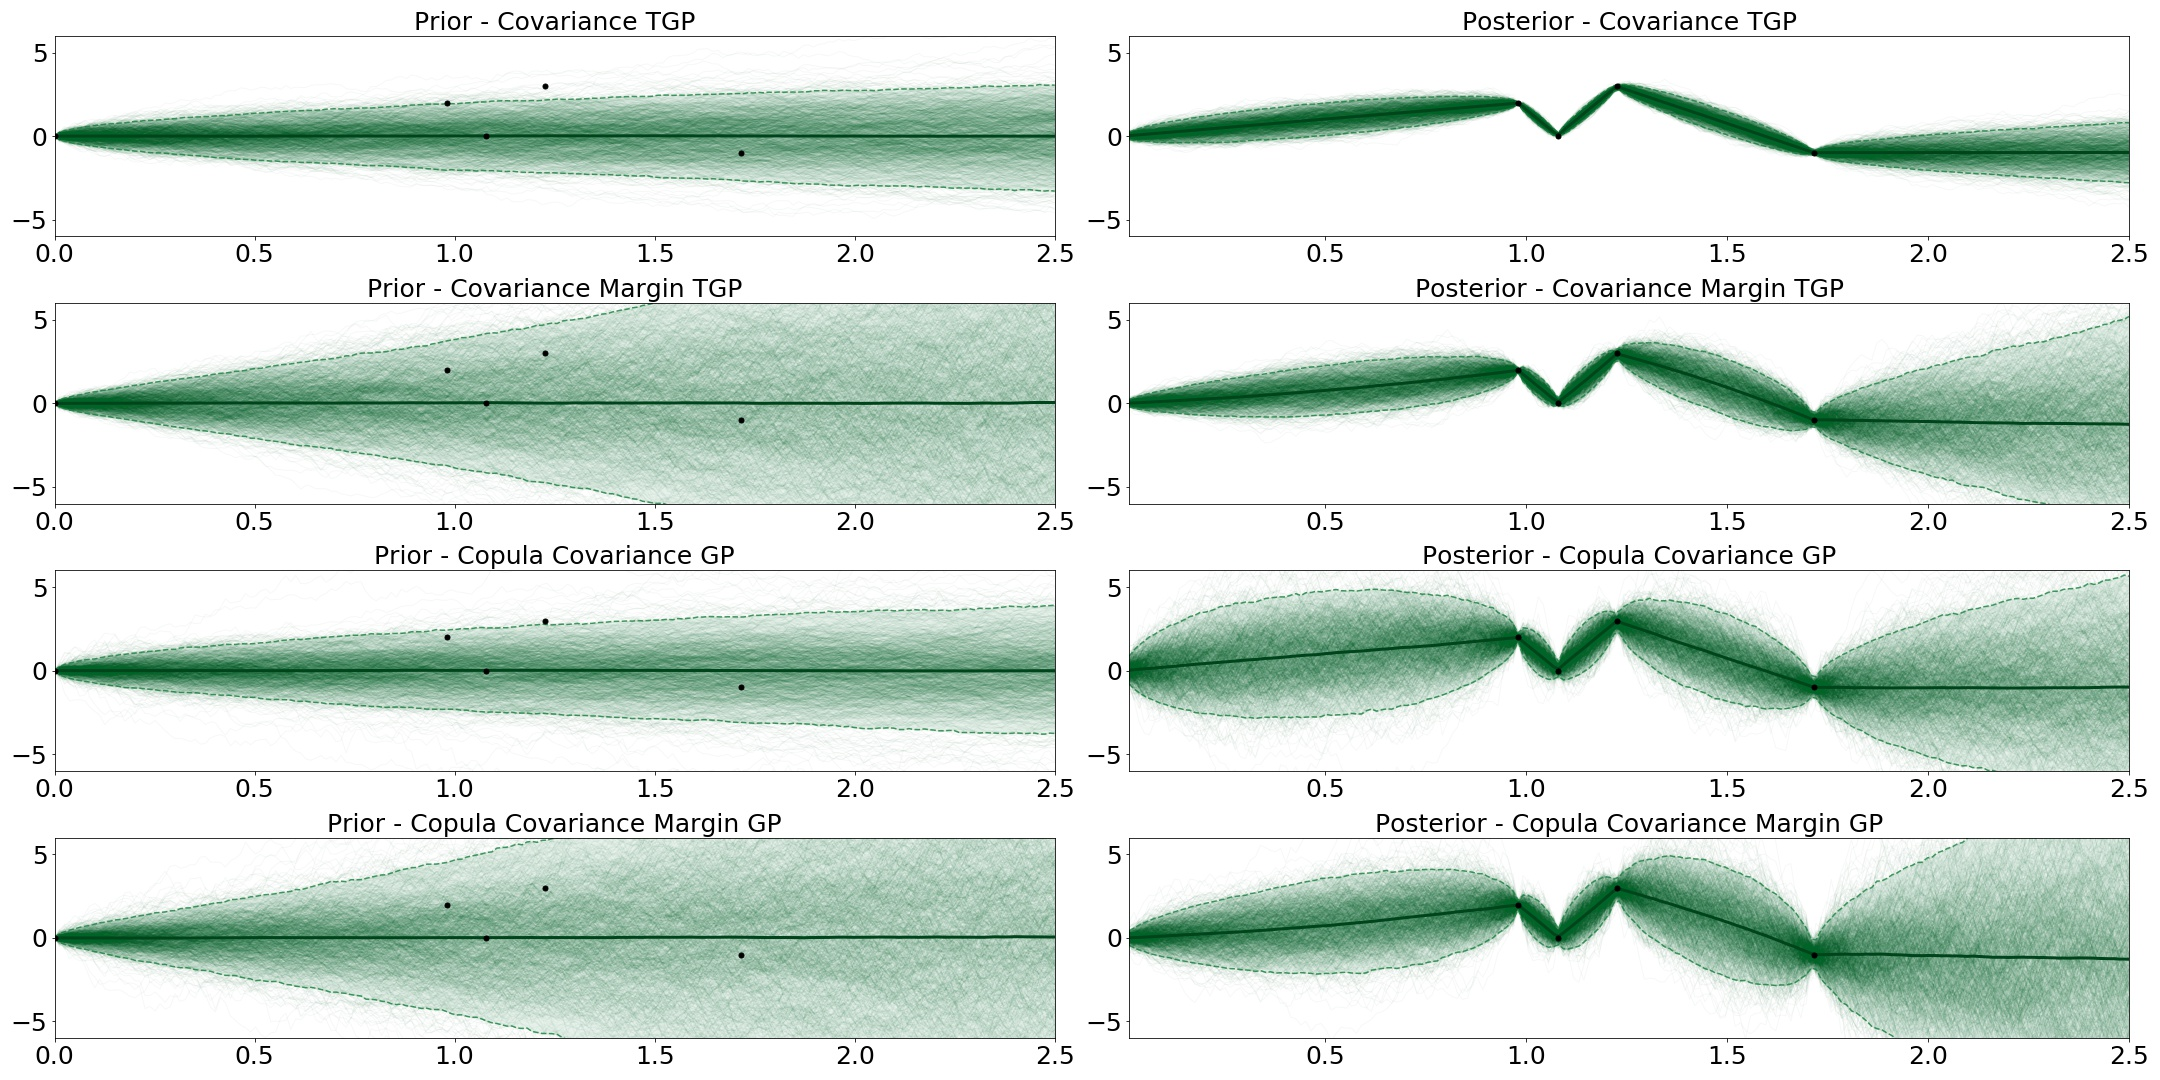
\includegraphics[width=0.9\textwidth]{tgp}
	\caption{Muestras de cuatro TGP: el primer y segundo ejemplos tienen cópula gaussiana, mientras que el tercero y cuarto tienen cópulas de \(t\) de Student.}
	\label{fig_tgp1}
\end{figure}


\section{Proceso Transportado Profundo}
\label{sec:computationtgp}
Tanto la generalidad como el cálculo factible del enfoque presentado basado en el transporte para la regresión no paramétrica nos motivan a definir modelos complejos inspirados en los avances recientes de la comunidad de aprendizaje profundo. Mediante la composición de transportes elementales (o \emph{capas}) podemos generar transportes más expresivos (o \emph{profundos}). En esta sección, explicaremos cómo construir dicha arquitectura, describiremos las propiedades que se heredan a través de la composición, para finalmente proponer familias de transportes que se pueden componer juntos y estudiar sus propiedades en el problema de regresión.



\subsection{Consistencia de un proceso transportado profundo}

En este artículo presentamos cuatro tipos de transportes, que pueden verse como \emph{capas} elementales para los modelos de regresión. Nuestro enfoque parte de una referencia de ruido blanco gaussiano \(f \sim \eta\), ya que es un proceso bien conocido con densidad explícita y métodos de muestreo eficientes. La primera capa determina la \emph{cópula} del proceso inducido (elíptica) mediante transportes elípticos. En el caso elíptico, es posible componerlo con un transporte de covarianza para determinar la correlación sobre el proceso estocástico inducido. Finalmente, en cualquier caso, podemos componer cualquier número de transportes marginales para definir una distribución marginal expresiva sobre el proceso estocástico inducido, como se muestra en el trabajo anterior \cite{cwgp}. Como vimos en las secciones anteriores, estas composiciones son lo suficientemente consistentes y expresivas como para incluir GP, GP alabeadas, procesos de Student-t, procesos elípticos y los que podríamos llamar \emph{procesos elípticos deformados}.


\subsection{Entrenamiento de un proceso transportado profundo}
Asumiendo \(T\#\eta = \pi\), donde \(T\) es una composición de \(k\) transportes, es decir \(T = T^{(k)} \circ ... \circ T^{(1)}\). Denotando \(\eta^{(0)}=\eta\) y asumiendo que cada \(\eta^{(j)}=T^{(j)}\#\eta^{(j-1)}\) es un proceso transportado con transportes finito dimensionales \(\{T_{\bft}^{(j)}\}_{j=1}^k\). Notemos que \(\eta^{(k)} = T\#\eta = \pi\), donde \(T_{\bft} = T_{\bft}^{(k)} \circ ... \circ T_{\bft}^{(1)}\) son transportes finito dimensionales con \(S_{\bft} = S_{\bft}^{(1)} \circ ... \circ S_{\bft}^{(k)}\). Como consecuencia, la composición de procesos transportados es un proceso transportado. En consecuencia, la NLL puede ser calculada como
\begin{align}
\label{eq:TGP_NLL2}
-\log \pi_{\bft}(\bfy|\theta) = -\log \eta_{\bft}(S_{\bft}(\bfy)) - \sum\nolimits_{j=1}^k \log |\nabla S_{\bft}^{(j)}(S_{\bft}^{[(j+1):k]}(\bfy))|,
\end{align}
donde \(S_{\bft}^{[j:k]}(\bfy) = S_{\bft}^{(j)} \circ ... \circ S_{\bft}^{(k)} (\bfy)\), con la convención \(S_{\bft}^{[(k+1):k]}(\bfy) = \bfy\). La fórmula anterior se basa en el cálculo de cada \(F_{\bft}^{(j)}(\bfz)= \log |\nabla S_{\bft}^{(j)}(\bfz)|\), que se puede calcular alternativamente como \(F_{\bft}^{(j)}(\bfz)=- \log |\nabla T_{\bft}^{(j)}(S_{\bft}^{(j)}(\bfz))|\), o, para el caso triangular y diagonal, como \(F_{\bft}^{(j)}(\bfz)=\sum_{i} \log \frac{\partial (S_{\bft})_i}{\partial y_i}(\bfz)\). El siguiente algoritmo calcula la NLL, sujeto a poder evaluar cada función \(F_{\bft}^{(j)}\) t \(S_{\bft}^{(j)}\).

\begin{algorithm}[!h]
	\caption{Calcula la NLL de un proceso transportado profundo}
	\label{algo1}
	\begin{algorithmic} 
		\Require Datos \((\bft,\bfy )\), transportes inversos \(T^{-1}_{\bft}(\bfz) = S_{\bft}^{(1)} \circ ... \circ S_{\bft}^{(k)}(\bfz)\) y \(F_{\bft}^{(j)}(\bfz)=\log |\nabla S_{\bft}^{(j)}(\bfz)|\).
		\Ensure  \(\mathcal{L} = -\log \pi_{\bft}(\bfy|\theta)\)
		\State \(\bfz \gets \bfy\), \(\mathcal{L} \gets 0\)
		\For{\( j \in k,...,1 \)}
		\State \(\mathcal{L} \gets \mathcal{L} - F_{\bft}^{(j)}(\bfz)\)
		\State \(\bfz \gets S_{\bft}^{(j)}(\bfz)\)
		\EndFor
		\State \(\mathcal{L} \gets \mathcal{L} - \log \eta_{\bft}(\bfz)\)
		\Return \(\mathcal{L}\)
	\end{algorithmic}
\end{algorithm}

\begin{remark}
	El algoritmo \ref{algo1} está basado en aplicar la regla de la cadena y el teorema de la función inversa sobre la composición de inversas \(S_{\bft} = S_{\bft}^{(1)} \circ ... \circ S_{\bft}^{(k)}\), entonces
	\begin{align}
	\nabla S_{\bft}(\bfy) &= \nabla S_{\bft}^{(1)}( S_{\bft}^{(2)} \circ ... \circ S_{\bft}^{(k)}) \nabla S_{\bft}^{(2)}( S_{\bft}^{(3)} \circ ... \circ S_{\bft}^{(k)}) .... \nabla S_{\bft}^{(k-1)}(S_{\bft}^{(k)}(\bfy))  \nabla S_{\bft}^{(k)}(\bfy),\\
	&= \nabla T_{\bft}^{(1)}( S_{\bft}^{(1)} \circ ... \circ S_{\bft}^{(k)})^{-1} \nabla T_{\bft}^{(2)}( S_{\bft}^{(2)} \circ ... \circ S_{\bft}^{(k)})^{-1} .... \nabla T_{\bft}^{(k)}(S_{\bft}^{(k)}(\bfy))^{-1}.
	\end{align}
\end{remark}

El algoritmo \ref{algo1} es computacionalmente eficiente en términos de uso mínimo de memoria (incluso la variable \(\bfz\) puede usar la misma memoria que \(\bfy\)), y se puede ejecutar en el menor tiempo posible llamando a cada función \(F_{\bft}^{(j)}\) y \(S_{\bft}^{(j)}\) solo una vez. Al implementar los cálculos de NLL en cualquier marco de tensor moderno, como PyTorch, es posible aplicar la diferenciación automática \cite{paszke2017automatic} para calcular la derivada de NLL con respecto a los parámetros. Además, este algoritmo es paralelizable en \(\theta\), lo que permite una evaluación eficiente de NLL para múltiples valores de \(\theta\) simultáneamente en arquitecturas como las GPU. Esta es una propiedad deseada para los métodos de optimización sin derivados, como la optimización de enjambres de partículas \cite{kennedy2010particle}, o los muestreadores de conjuntos MCMC \cite{goodman2010ensemble}. En los métodos de descenso de gradiente estocástico \cite{bottou2010large}, dado que en cada paso usamos un submuestreo de los datos, podemos aprovechar las arquitecturas basadas en GPU que se ejecutan en múltiples ejecuciones paralelas, para navegar mejor en el espacio de los modelos.


\subsection{Inferencia de un proceso transportado profundo}

Como la operación de composición conserva la triangularidad, asumimos que \(T^{(j)}\) son triangulares para \(j > l\), además de poder calcular la parte posterior de \(\eta^{(l)}\), es decir, calcular \(\eta_{\bfto|\bft}^{(l)}(\cdot|\bfx)\) para cualquier entrada \(\bfto\). Sin pérdida de generalidad, se puede suponer que \(l = 1\), ya que es posible colapsar por composición los transportes de \(l\) en uno solo. El siguiente algoritmo genera muestras de la distribución posterior \(\pi_{\bfto|\bft}(\bfyo|\bfy)\) bajo los supuestos anteriores.

\begin{algorithm}[!h]
	\caption{Generar muestras desde la posterior}
	\label{algo2}
	\begin{algorithmic} 
		\Require Observaciones \(\bfy \sim \pi_{\bft}\), nuevas entradas \(\bfto \in \calI^d, d \in \mathbb{N}\), número de muestras \(N \in \naturals\).
		\Ensure  \(\bfyo_i \sim \pi_{\bfto|\bft}(\bfyo|\bfy)\) para \(i=1,...,N\)
		\State \(\bfx \gets S_{\bft}^{[l+1:k]}(\bfy)\)
		\State \(R(\cdot) \gets P_{\bfto} \circ T_{\bft,\bfto}^{[l+1:k]}(\bfx, \cdot)\)
		\For{\( i \in 1,...,N \)}
		\State \(\bfxo_i \sim \eta_{\bfto|\bft}^{(l)}(\cdot|\bfx)\)
		\State \(\bfyo_i \leftarrow R(\bfxo_i)\)
		\EndFor
		\Return \(\{\bfyo_1,...,\bfyo_N\}\)
	\end{algorithmic}
\end{algorithm}

El algoritmo \ref{algo2} es paralelizable en \(N\), ya que la función \(R(\cdot)\) es la misma para todas las muestras, y por lo tanto nos permite obtener múltiples muestras simultáneamente de manera eficiente. Este puede ser utilizado a su vez para calcular momentos, cuantiles u otras estadísticas de forma empírica a través de Monte Carlo.

\subsection{Capa ruidosa}

Bajo la presencia de observaciones ruidosas, siguiendo la misma lógica que los GPs, warped GPs \cite{snelson2004warped} y los procesos Student-t \cite{shah2014student}, consideramos que el transporte de covarianza tiene un comportamiento especial. Sea \(k(t,s) = r(t,s) + \sigma_0\delta_{t,s}\), donde \(\delta\) es delta de Kronecker, \(\sigma_0\) es el parámetro que controla la intensidad del ruido y \(r(t,s)\) es la función de covarianza libre de ruido. Consideramos que las observaciones tienen ruido no correlacionado. Mientras que para el entrenamiento usamos \(k(t,s)\) en la fórmula de NLL, en la inferencia usamos \(k(t,s)\) en el paso hacia atrás (es decir, para el mapa inverso \(\bfx = T_{\bft }^{-1}(\bfy)\)), y en el paso hacia adelante (es decir, para impulsar la distribución de referencia) usamos \(r(t,s)\), en lugar de \(k(t,s)\) , para realizar una predicción de ruido libre.


\subsection{Sparse layer}
Mientras que los transportes marginales y de cópula se pueden evaluar de manera eficiente sin necesidad de datos de entrenamiento, los transportes de covarianza necesitan todos los datos \(\bfy\) para la inferencia de rendimiento. La complejidad computacional de la evaluación es \(\O(n^2)\) en memoria y \(\O(n^3)\) en tiempo, donde \(n=|\bfy|\). Las aproximaciones dispersas se usan ampliamente para resolver este problema en los GP \cite{quinonero2005unifying, snelson2006sparse, titsias2009variational}, y es natural definir un transporte \emph{sparse} como \(T_{\bfto}(\bfu) = \Sigma_{\ bfto\bfs}\Sigma_{\bfs\bfs}^{-1}\bfz + \chol(\Sigma_{\bfto\bfto} - \Sigma_{\bfto\bfs}\Sigma_{\bfs\bfs}^{ -1}\Sigma_{\bfto\bfs})\bfu\), donde \((\bfs,\bfz)\) son pseudodatos entrenables con \(|\bfs| = m < n\). El entrenamiento de pseudodatos sigue las mismas ideas que los GP dispersos, como las aproximaciones SoD y SoR \cite{quinonero2005unifying}, donde el costo computacional cae a \(\O(nm)\) en el espacio y \(\O(nm^2)\) a tiempo.


\section{Validación Experimental}
\label{sec:experimentstgp}

\comment{le cambiaria el nombre a algo asi como: 'aplicación' o ejemplo, porque como es algo ya establecido no deberia ser una validación}

Validamos nuestro enfoque con tres series de tiempo del mundo real, descritas a continuación:
\begin{enumerate}
	\item \textbf{Datos de manchas solares}: La serie temporal de manchas solares \cite{sunspots} corresponde al número anual de manchas solares entre 1700 y 2008, lo que da como resultado 309 puntos de datos, uno por año. Estas medidas son positivas y semiperiódicas, con un ciclo de alrededor de 11 años.
	\item \textbf{Datos de frecuencia cardíaca}: Esta es una serie temporal de frecuencia cardíaca de la base de datos MIT-BIH (ecg.mit.edu) \cite{glass2012theory}. Esta serie contiene 1800 mediciones positivas espaciadas uniformemente de la frecuencia cardíaca instantánea (en unidades de latidos por minuto) de un solo sujeto, que ocurren a intervalos de 0,5 segundos y muestran un patrón semiperiódico. Para problemas de rendimiento, tomamos una submuestra de 450 medidas en intervalos de 2,0 segundos.
	\item \textbf{Datos económicos}: Esta serie de tiempo corresponde al promedio trimestral \emph{3-Month Treasury Bill: Secondary Market Rate} \cite{tb3ms} entre el primer trimestre de 1959 y el tercer trimestre de 2009, es decir, 203 observaciones, una por trimestre. Sabemos de antemano que esta señal macroeconómica es el precio de los bonos libres de riesgo del gobierno estadounidense, que no pueden tomar valores negativos y pueden tener grandes desviaciones positivas.
\end{enumerate}

Debido a la naturaleza semiperiódica de la serie temporal, consideramos una mezcla espectral ruidosa con dos componentes kernel \(k_{SM}\) \cite{wilson2013gaussian} para el transporte de covarianza. Dado que las series de tiempo son positivas, usamos una deformación de Box-Cox desplazada \(\phi_{BC}\) \cite{rios2018learning} para el transporte marginal. Comparamos dos modelos: un GP distorsionado, con \(k_{SM}\) kernel y \(\phi_{BC}\) warping; y un TGP con un transporte de cópula Student-t, además de los transportes marginales y de covarianza descritos anteriormente.

Dejamos los GP estándar fuera del experimento ya que la suposición de gaussianidad viola la naturaleza de los conjuntos de datos, ya que tiene un poder predictivo más bajo que el WGP, como se muestra en \cite{rios2018learning, riostobar2019cwgp}. Para ilustrar este hecho, en la Fig. \ref{fig_sunspots} mostramos la parte posterior de tres modelos entrenados: GP en azul, WGP en verde y TGP en morado. Graficamos las observaciones (puntos negros), la media (línea continua), el intervalo de confianza de 95\textbf{\%} (línea discontinua) y 25 muestras (líneas borrosas). Observe cómo el GP falla al modelar la positividad y la amplitud correcta de los fenómenos.

\begin{figure}
	\centering
	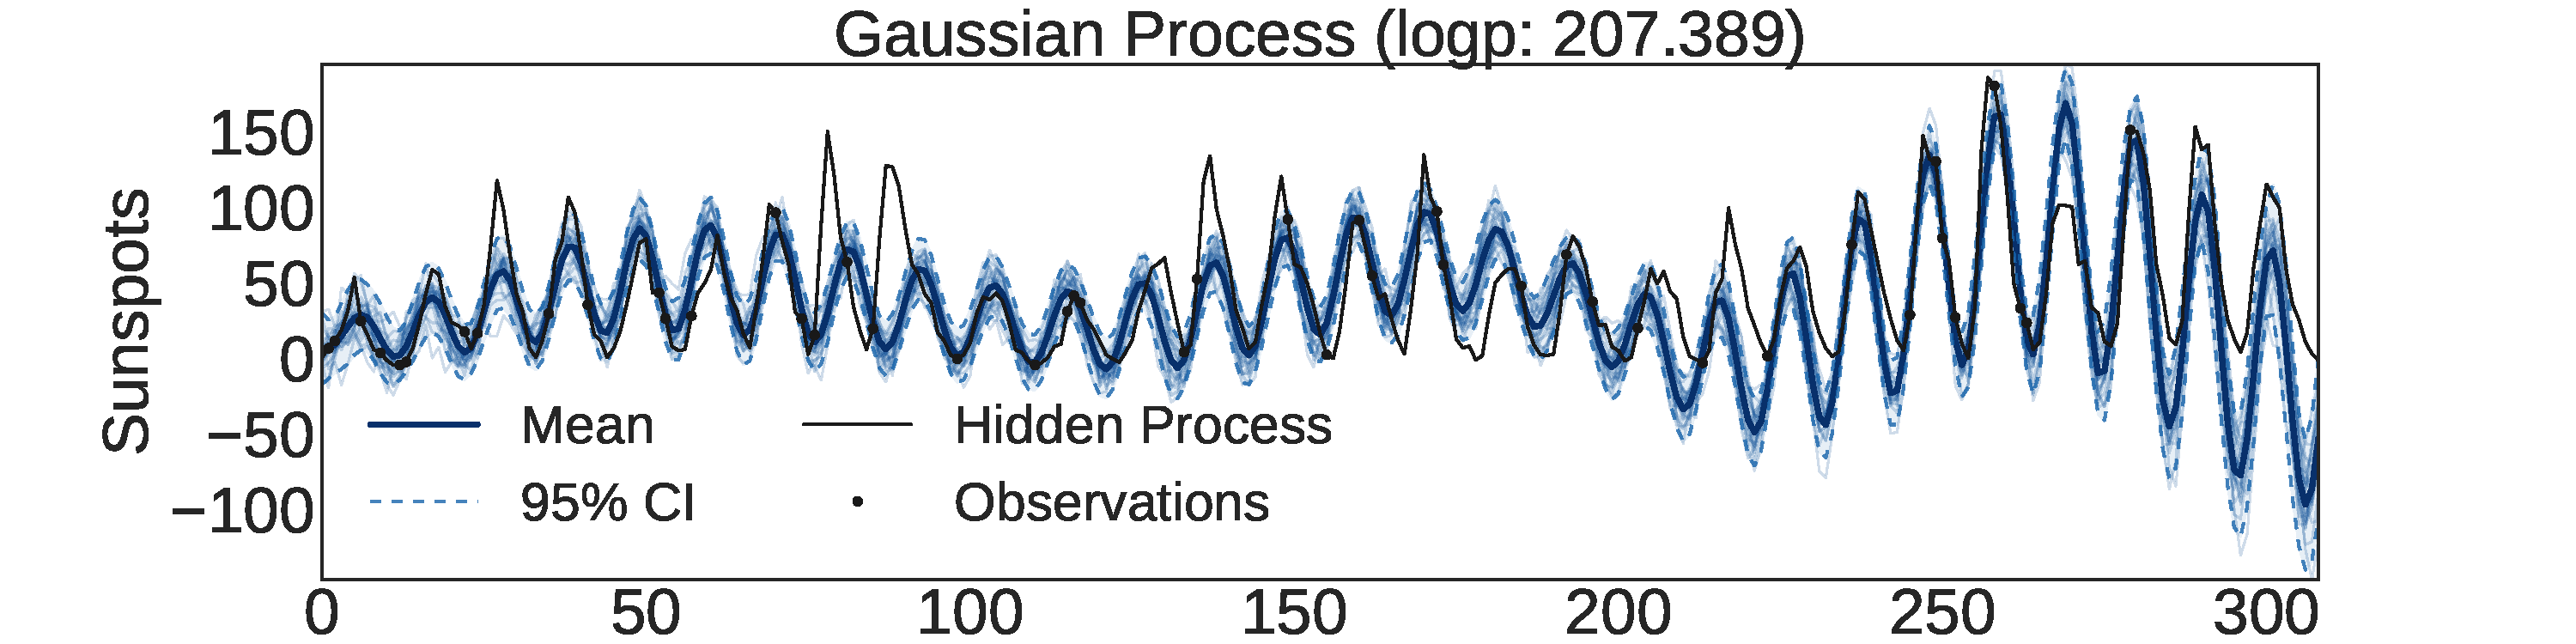
\includegraphics[width=0.7\textwidth]{example_sunspots_gp}
	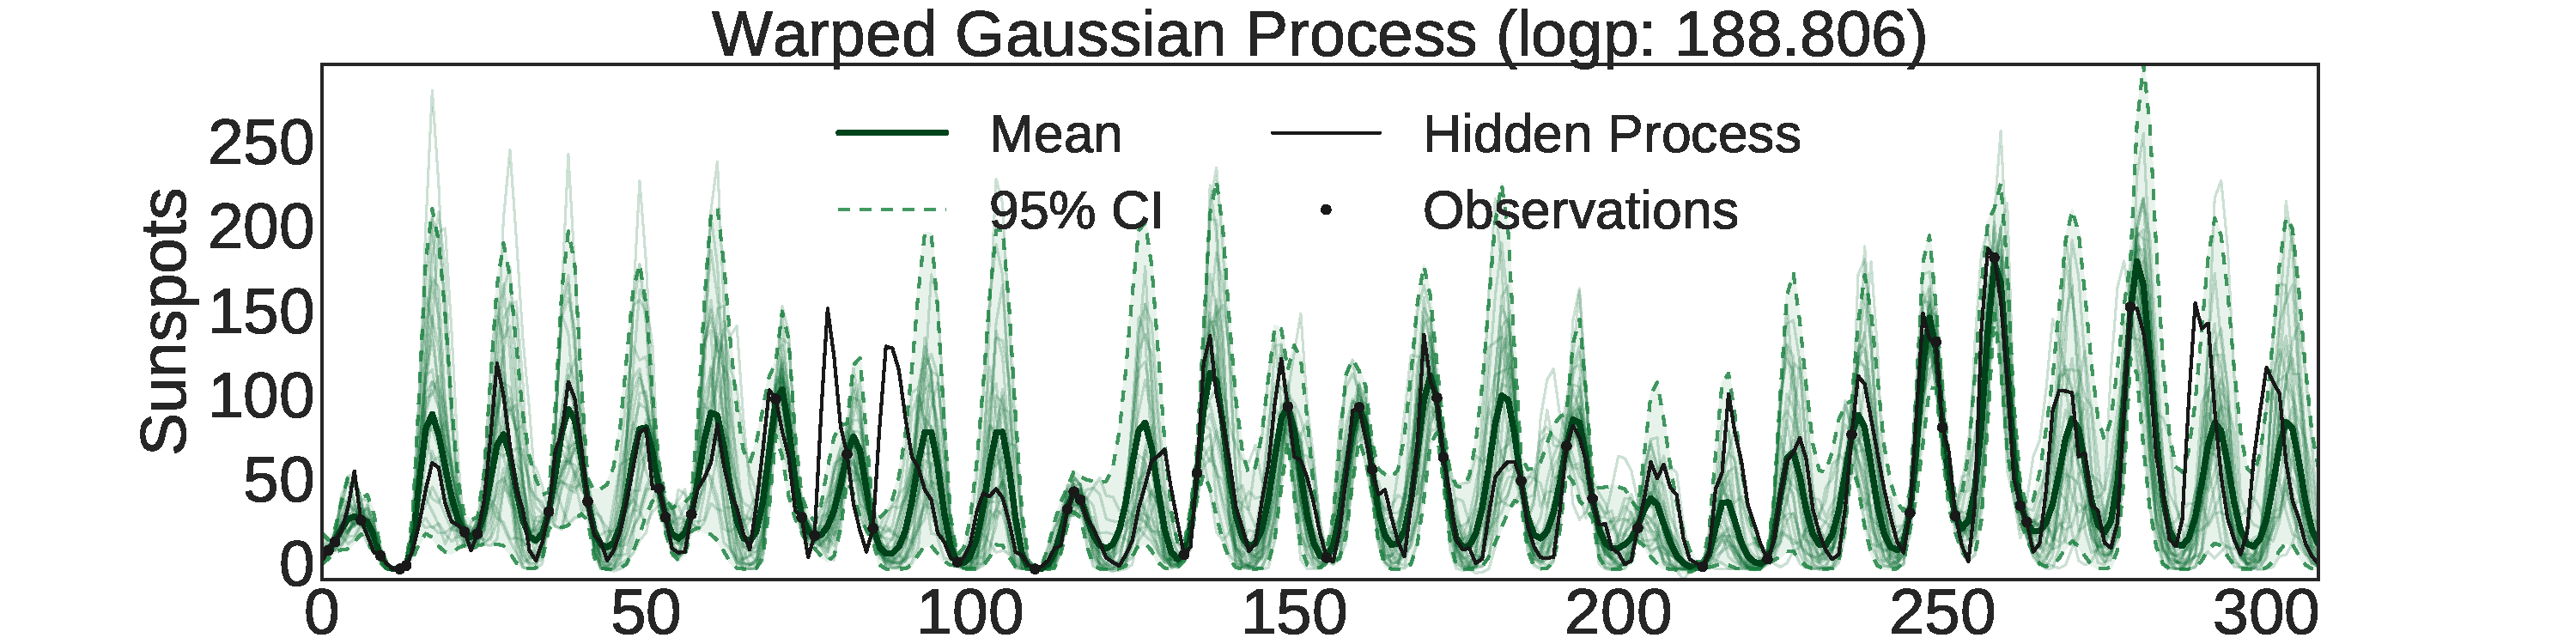
\includegraphics[width=0.7\textwidth]{example_sunspots_wgp}
	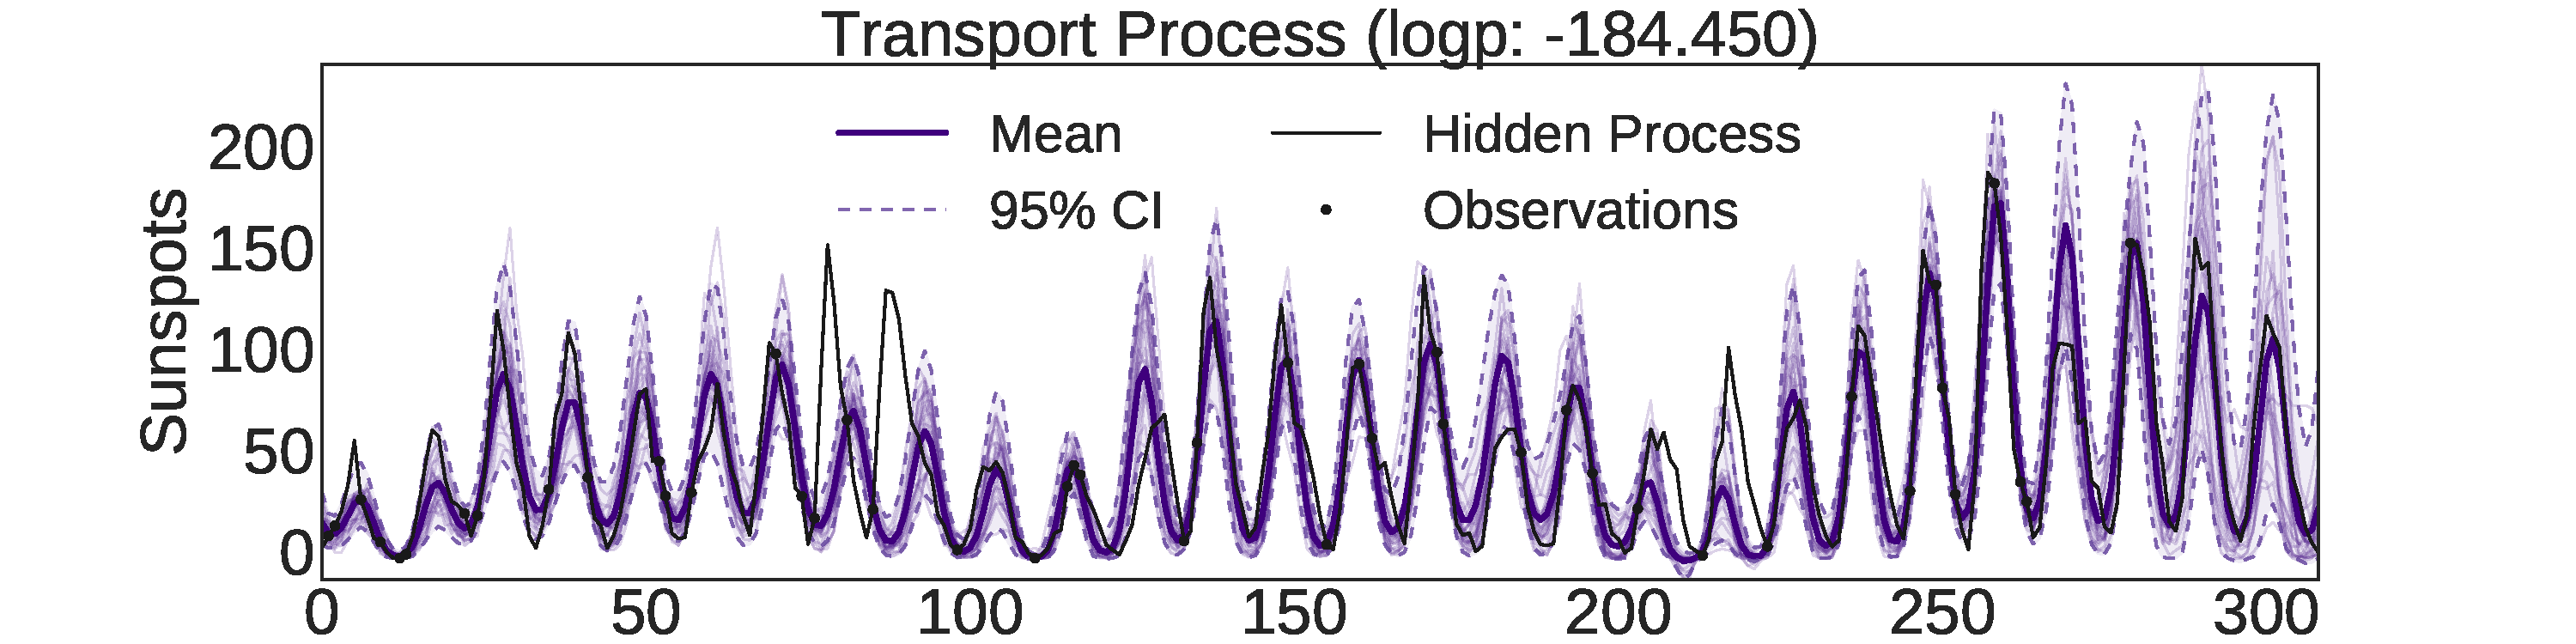
\includegraphics[width=0.7\textwidth]{example_sunspots_tgp}
	\caption{GP (azul), WGP (verde) y TGP (púrpura) sobre los datos de manchas solares.}
	\label{fig_sunspots}
\end{figure}


\begin{table}
	\centering
	\tiny
	\begin{tabular}{l|ll|ll|ll}
		\toprule
		{} & \multicolumn{2}{l}{Manchas Solares} & \multicolumn{2}{l}{Frecuencia Cardíaca} & \multicolumn{2}{l}{Económica} \\
		{} &                      WGP &                      TGP &                 WGP &                 TGP &                WGP &                TGP \\
		\midrule
		MAE &       25.266 \(\pm\) 4.607 &       24.710 \(\pm\) 4.271 &   2.965 \(\pm\) 0.827 &   2.907 \(\pm\) 0.715 &  1.132 \(\pm\) 0.260 &  1.111 \(\pm\) 0.215 \\
		EAE &       30.166 \(\pm\) 4.374 &       29.649 \(\pm\) 4.168 &   3.431 \(\pm\) 0.732 &   3.388 \(\pm\) 0.660 &  1.392 \(\pm\) 0.235 &  1.380 \(\pm\) 0.206 \\
		MSE &  1,306.253 \(\pm\) 560.496 &  1,223.257 \(\pm\) 421.385 &  16.405 \(\pm\) 8.809 &  15.740 \(\pm\) 7.619 &  3.002 \(\pm\) 1.643 &  2.860 \(\pm\) 1.311 \\
		ESE &  1,889.318 \(\pm\) 633.325 &  1,796.989 \(\pm\) 514.193 &  21.963 \(\pm\) 8.524 &  21.554 \(\pm\) 8.213 &  4.376 \(\pm\) 1.725 &  4.272 \(\pm\) 1.424 \\
		\bottomrule
	\end{tabular}
	\vspace{0.5em}
	\caption{WGP and TGP results over Sunspots, Heart and Economic datasets.}
	\label{tab:table_results} 
\end{table}


El experimento se implementó en una biblioteca basada en Python llamada \emph{tpy: Transport Processes in Python}\cite{tpy}, con un backend de PyTorch para compatibilidad con GPU y diferenciación automática \cite{paszke2017automatic}. El entrenamiento se realizó minimizando el NLL de eq.~\eqref{eq:TGP_NLL2}, a través de un método rprop de mini lotes estocásticos \cite{riedmiller1993direct}, para luego terminar con iteraciones no estocásticas.

En cada experimento, seleccionamos al azar (uniformemente) 15\text{\%} de los datos para entrenamiento y los 85\text{\%} restantes para validación. Dados los puntos de datos de validación \(\{y_i\}_{i=1}^n\), para cada modelo generamos \(S\) muestras \(\{y_i^{(k)}\}_{i=1}^n \) para \(k=1,...,S\), y luego calculamos cuatro índices de rendimiento: el error cuadrático medio como \(\text{MSE} = \frac{1}{n}\sum\limits_{i=1 }^{n}\left(y_{i} - \frac{1}{S}\sum_{k=1}^{S}y_i^{(k)}\right)^2\), el error absoluto medio como \(\text{MAE} = \frac{1}{n}\sum\limits_{i=1}^{n}|y_{i} - \frac{1}{S}\sum_{k=1} ^{S}y_i^{(k)}|\), el error cuadrado esperado como \(\text{ESE} = \frac{1}{n}\sum\limits_{i=1}^{n}\frac{ 1}{S}\sum_{k=1}^{S}(y_{i} - y_{i}^{(k)})^2\), y el error absoluto esperado como \(\text{EAE} = \frac{1}{n}\sum\limits_{i=1}^{n}\frac{1}{S}\sum_{k=1}^{S}|y_{i} - y_{i} ^{(k)}|\). Repetimos cada experimento 100 veces. Los resultados de todos estos experimentos se resumen en la Tabla 1, que muestra cada media y desviación estándar. Consistentemente, el TGP propuesto tiene un mejor rendimiento que la alternativa de warped GP, para cada conjunto de datos e índice de evaluación.

\comment{parrafo: concluir y aterrizar los conceptos mencionados, generar una pequeña discusión sobre aplicaciones, limitantes y demasese. motivar la lectura tanto de otros capitulos como de demás literatura}